\documentclass[11pt,a4paper]{article}

\usepackage[T1]{fontenc}
\usepackage[utf8]{inputenc}
\usepackage[margin=2.4cm]{geometry}
\usepackage{graphicx}
\usepackage{amsmath,amssymb}
\usepackage{bm}
\usepackage{hyperref}
\usepackage{xcolor}
\usepackage{siunitx}
\usepackage{booktabs}
\usepackage{natbib}
\usepackage{caption}

\captionsetup{font=small,labelfont=bf,labelsep=period,justification=raggedright,singlelinecheck=false}

\hypersetup{colorlinks=true, linkcolor=blue!50!black, citecolor=blue!50!black, urlcolor=blue!50!black}

\graphicspath{{../figures/}}

\begin{document}

\title{A two-feedback Vicsek-Couzin flock: density-stratified heading correlations as the scale-invariant fingerprint of motility--noise coupling}

\author{Yaya Youssouf Yaya \\[0.5em]
        \small D\'epartement de Math\'ematiques, \'Ecole Normale Sup\'erieure de
               N'Djam\'ena, BP~206, N'Djam\'ena, Tchad \\
        \small Chercheur Associ\'e, LMA, U.F.R.~Sciences et Technologies,
               Universit\'e Assane Seck de Ziguinchor, BP~523, Diabir,
               Ziguinchor, S\'en\'egal \\
        \small \texttt{yy.y@zig.univ.sn} \;\;
               ORCID: \href{https://orcid.org/0000-0003-0781-4923}{0000-0003-0781-4923}}

\date{\today}

\maketitle

\begin{abstract}
In the standard Vicsek model the self-propulsion speed and
the angular-noise distribution are global constants. Two
strands of the active-matter literature have softened each
of them in turn. A density-dependent speed is enough to
drive motility-induced phase separation, and heavy-tailed
L\'evy reorientations reshape the order--disorder
transition; what neither strand has resolved is what
happens when the two adaptations operate together. We close
that gap by gating both the speed and the stability index
of an $\alpha$-stable angular kick through one shared
sigmoid in the local neighbour count, so crowded particles
are simultaneously slow and Gaussian-like while isolated
ones are fast and Cauchy-like. A controlled seven-size
finite-size scaling against the original Vicsek model and
three single-channel ablations separates the two regimes
cleanly. Only the motility-active modes develop a critical
susceptibility scaling; the three fixed-noise-shape modes
plateau with slopes statistically indistinguishable from
zero. The full model is super-additive on this slope with
respect to the motility-only ablation, and the synergy
persists across all cumulative size budgets. The
density-stratified heading correlation inside the dense
phase, its dynamic counterpart $C(\tau)$, and the
maximum-cluster size all converge on the same picture: the
noise-shape feedback rectifies Cauchy bursts into
Gaussian-like kicks inside the motility-driven dense phase,
and the two channels cooperate super-additively. A
decoupled-sigmoid sweep on a $25$-cell threshold grid
shows that the motility threshold alone controls the sign
and amplitude of the rectification, while the noise-shape
threshold is essentially passive.
\end{abstract}

\section*{Highlights}
\begin{itemize}\setlength{\itemsep}{1pt}
  \item We resolve a regime previously studied only in
        isolation --- density-dependent motility and
        heavy-tailed L\'evy reorientations --- by activating
        both feedbacks in the same Vicsek--Couzin flock through
        a shared sigmoid.
  \item Heavy-tailed reorientations on their own do not
        drive a critical $\chi_{\max}(L)$ scaling on the
        seven-size lever; only the motility channel does, and
        the noise-shape adaptation adds super-additively on
        top of it.
  \item The density-stratified heading correlation inside
        the dense phase records the rectification with high
        precision ($\Delta g \simeq +0.15$, $z \simeq +14$
        at $L = 30$); its dynamic counterpart $C(\tau)$ holds
        the same gap over four decades in lag.
  \item A $25$-cell decoupled-sigmoid sweep shows the motility
        threshold $n_\star^v$ alone controls the sign and
        magnitude of the rectification ($R^2 = 0.88$ on
        $n_\star^v$, $R^2 = 0.04$ on the noise-shape
        threshold); the density-triggered slowdown is a
        necessary precondition for the heavy-tailed noise
        rectification to add coherence rather than destroy it.
\end{itemize}

\section{Introduction}

The diagnostic toolbox most often applied to self-propelled
flocks reads the order parameter and its global fluctuations.
The Vicsek model \citep{Vicsek1995} keeps two ingredients of
that flock --- metric alignment with neighbours and an
external angular noise --- and freezes everything else: every
particle moves at the same speed $v_0$, and every angular
kick is drawn from the same Gaussian. Both choices are
convenient. Both are physically wrong in interesting ways.
Self-propulsion speed responds to local crowding in essentially
every system one might want to model. Confluent epithelia jam
and arrest \citep{Bi2016}, swarming bacteria switch between
planktonic and biofilm regimes through quorum sensing, and
traffic flows of vehicles, pedestrians or migrating animals
all carry a marked speed--density anti-correlation
\citep{Greenshields, LWR}. The reorientation statistics are
no closer to Gaussian: heavy-tailed L\'evy turns have been
documented in foragers, T-cells and swarming bacteria
\citep{Reynolds2018, Harris2012, Ariel2015}. The biologically
honest model therefore lets both inputs depend on the local
environment, and the question we ask here is what such a
double dependence does to the dense phase that the alignment
interaction otherwise tries to build.

The two relaxations of the canonical model live in different
parts of the active-matter literature. Cates and Tailleur
\citep{CatesTailleur2015} proved that a density-dependent
speed $v(\rho)$ with $\partial \ln v / \partial \ln \rho < -1$
is enough to drive motility-induced phase separation (MIPS),
in which a dense slow phase coexists with a dilute fast
phase even with no alignment interaction at all. Heavy-tailed
angular noise has been studied on a separate track and is
known to reshape the order--disorder transition of metric
Vicsek dynamics. To our knowledge, the regime in which both
adaptations are switched on together has not been resolved.
The question is not academic. The angular-noise distribution
sets how particles escape spatial structures, while the
density-dependent speed sets those structures in the first
place, and the two channels therefore interrogate each other
inside the same dense regions.

We tie the two adaptations together in the simplest way
available. A single sigmoid in the local neighbour count
$n_i$ gates both the self-propulsion speed and the
angular-noise stability index, so that a crowded particle is
simultaneously slow and Gaussian and an isolated particle is
simultaneously fast and Cauchy. Switching both channels off
($v_i \equiv v_0$, $\alpha_i \equiv 2$) recovers the original
Vicsek dynamics, against which we benchmark at every step.
Two single-channel ablations isolate the individual
contributions: a motility-only mode with adaptive $v_i$ and
fixed Cauchy $\alpha = 1$, and a noise-shape-only mode with
fixed $v_i = v_{\max}$ and adaptive $\alpha_i \in [1, 2]$.

A short quantitative preview helps place the results that
follow. The finite-size scan covers $L \in \{15, 22, 30, 45,
64, 90, 128\}$ at fixed density $\sigma = N/L^2 = 2.22$. The
density-separation index $s_{\rm sep}$, the standard MIPS
diagnostic, plateaus at $\simeq 1.70$ at the largest sizes
for both the motility-only ablation and the double-adaptive
model, against $1.13$--$1.16$ for the original Vicsek
reference, the heavy-tailed Cauchy reference, and the
noise-shape-only ablation: only the two motility-active modes
produce spatial phase separation. A log--log fit of the
susceptibility scaling $\chi_{\max} \sim L^{a}$ on the seven
sizes gives $a_{\rm Vicsek} = +0.01$, $a_{\rm Cauchy} =
-0.12$, $a_{\rm noise} = +0.00$, $a_{\rm motility} = +2.34$,
and $a_{\rm full} = +2.95$. The separation between modes is
qualitative, not just quantitative. The three fixed-noise-shape
modes (Vicsek--Gaussian, Cauchy reference, noise-shape-only
ablation) all carry slopes statistically indistinguishable
from zero, with the Cauchy reference robustly negative
($95\%$ bootstrap CI $[-0.15, -0.08]$); only the two
motility-active modes develop a critical $\chi_{\max}(L)$
scaling. The synergy diagnostic
$\Delta = (a_{\rm full} - a_{\rm Cauchy})
- (a_{\rm noise} - a_{\rm Cauchy})
- (a_{\rm motility} - a_{\rm Cauchy})$
would vanish for two channels combining linearly above the
Cauchy backdrop. Instead it traces a persistently positive
trajectory across the cumulative size budget:
$\Delta_4 = +0.69$ on the four smallest sizes,
$\Delta_5 = +1.45$ once $L = 64$ is folded in,
$\Delta_6 = +0.46$ at $L = 90$, and $\Delta_7 = +0.48$ at
$L = 128$. The Cauchy-only modes contribute essentially no
susceptibility scaling on their own, so $\Delta$ is dominated
by the difference between the full and motility-only slopes,
$a_{\rm full} - a_{\rm motility} \simeq +0.6$, well outside
the bootstrap envelope of zero on the four smallest sizes.
The signal persists through seven sizes: the noise-shape
feedback adds super-additively to the motility-driven critical
scaling rather than washing out in the asymptotic regime.

The mechanism behind these numbers is direct. Inside the
dense phase that the motility channel produces, the shared
sigmoid pushes the local stability index toward
$\alpha_{\max} = 2$, and the Cauchy bursts that would
otherwise scramble local alignment are rectified into
Gaussian-like kicks. The dense-quartile heading correlation
records the rectification cleanly: at $L = 30$, a ten-seed
measurement gives $g(r \simeq 0.6) = 0.542 \pm 0.007$ in the
motility-only ablation against $0.695 \pm 0.008$ in the
double-adaptive model, a paired gap of $+0.153 \pm 0.011$
($z = +13.6$). The dilute-quartile correlation, by contrast,
is essentially insensitive to the rectification and stays
near zero in both modes; the noise-shape adaptation acts only
where the shared sigmoid sends it, in the dense phase where
particles are slow and crowded. The cluster diagnostics
sharpen the geometric picture. At $L = 30$, the
double-adaptive model produces $162.0 \pm 14.5$ dense
clusters per snapshot against $187.9 \pm 12.3$ in the
motility-only ablation, a paired difference of
$-25.9 \pm 22.6$ ($z = -1.15$, not significant); but the
maximum-cluster size is markedly larger in the double-adaptive
model, at $176.6 \pm 42.3$ particles versus $55.0 \pm 7.5$ in
motility-only ($z = +2.7$). The rectification therefore fuses
dense patches into a few large droplets rather than
multiplying smaller ones. A two-dimensional decoupled-sigmoid
sweep (Sec.~\ref{sec:decoupled}) sharpens the picture by
exposing the dominant control variable. On a $25$-cell grid
$(n_\star^v, n_\star^\alpha) \in \{1, 2, 3, 5, 8\}^2$ the
sign and amplitude of the dense-quartile gap are governed
almost entirely by the motility threshold $n_\star^v$: a
linear regression captures $R^2 = 0.88$ on $n_\star^v$ alone
with $\Delta g \simeq -0.144\,n_\star^v + 0.52$, while the
analogous fit on the noise-shape threshold $n_\star^\alpha$
captures only $R^2 = 0.04$. The biological reading is
unambiguous: the density-triggered slowdown is a necessary
precondition; without it, the heavy-tailed noise rectification
damages dense-phase coherence instead of building it.

\section{Model and methods}

\subsection{Dynamics}

We work with $N$ point particles in a square box of side $L$
with periodic boundary conditions. Particle $i$ carries a
position $\mathbf x_i \in [0, L)^2$ and a heading
$\theta_i \in (-\pi, \pi]$, advanced synchronously through
\begin{equation}
\theta_i(t+1) = \theta_i^\star(t+1) + \xi_i(t),
\qquad
\mathbf x_i(t+1) = \mathbf x_i(t) + v_i(t+1)\,\vec e_i(t+1)
   \pmod L,
\label{eq:update}
\end{equation}
with $\vec e_i = (\cos\theta_i, \sin\theta_i)$. The desired
heading $\theta_i^\star$ follows the Couzin priority rule
\citep{Couzin2002}, made explicit by introducing the
repulsion set $\mathcal R_i = \{j \neq i : |\mathbf r_{ij}|
< R_r\}$ with $\mathbf r_{ij} = \mathbf x_j - \mathbf x_i$,
and the alignment set
$\mathcal A_i = \{j \neq i : R_r \le |\mathbf r_{ij}| < R_a\}$.
Each particle senses omnidirectionally: every neighbour in the
repulsion disc or the alignment annulus enters the
corresponding set, regardless of its angular position relative
to $\vec e_i(t)$. Repulsion takes priority over alignment,
and alignment over inertia:
\begin{equation}
\theta_i^\star(t+1) =
\begin{cases}
\arg\!\left(-\sum_{j \in \mathcal R_i}
   \mathbf r_{ij} / |\mathbf r_{ij}|\right),
   & \mathcal R_i \neq \emptyset, \\[4pt]
\arg\!\left(\sum_{j \in \mathcal A_i} e^{i\theta_j(t)}\right),
   & \mathcal R_i = \emptyset
   \text{ and } \mathcal A_i \neq \emptyset, \\[4pt]
\theta_i(t),
   & \mathcal R_i = \mathcal A_i = \emptyset.
\end{cases}
\label{eq:theta_star}
\end{equation}
The three branches respectively send the particle away from
the centroid of its repulsion-zone neighbours, align it with
the mean heading of its alignment-zone neighbours, and
preserve its current heading when no neighbour is present.
Interactions run in $O(N)$ on a cell-list partition.

The angular kick $\xi_i$ is a symmetric $\alpha$-stable variate
with the stability index set particle by particle,
\begin{equation}
\xi_i(t) \sim S_{\alpha_i(t)}\bigl(c = \eta,\, \beta_{\rm stab}
   = 0,\, \mu = 0\bigr),
\label{eq:noise}
\end{equation}
which we sample with the Chambers--Mallows--Stuck representation
\citep{Chambers1976} from a uniform $U$ and an exponential $W$.
The Gaussian limit $\alpha_i = 2$ is handled separately and
recovers the original Vicsek noise.

\subsection{The shared sigmoid}

The single departure from canonical Vicsek dynamics is that
both the propulsion speed and the noise stability index become
local fields, both controlled by the same instantaneous
neighbor count $n_i(t) = |\mathcal A_i(t)|$ through one
sigmoid,
\begin{align}
\sigma_i(t) & = \frac{1}{1 + \exp\bigl[-s\,(n_i(t) -
   n_\star)\bigr]},
\label{eq:sigmoid} \\
v_i(t) & = v_{\max} - (v_{\max} - v_{\min})\,\sigma_i(t),
\label{eq:v_adapt} \\
\alpha_i(t) & = \alpha_{\min} + (\alpha_{\max} - \alpha_{\min})
\,\sigma_i(t).
\label{eq:alpha_adapt}
\end{align}
A crowded particle ($n_i \gg n_\star$) sits at $\sigma_i \to
1$, hence at $v_i \to v_{\min}$ and $\alpha_i \to
\alpha_{\max} = 2$. An isolated particle ($n_i \ll n_\star$)
sits at $\sigma_i \to 0$, $v_i \to v_{\max}$, and $\alpha_i
\to \alpha_{\min} = 1$. The two channels are locked: slow
means Gaussian, fast means Cauchy. No operating point lets
them fight each other locally.

\begin{figure}[!ht]
    \centering
    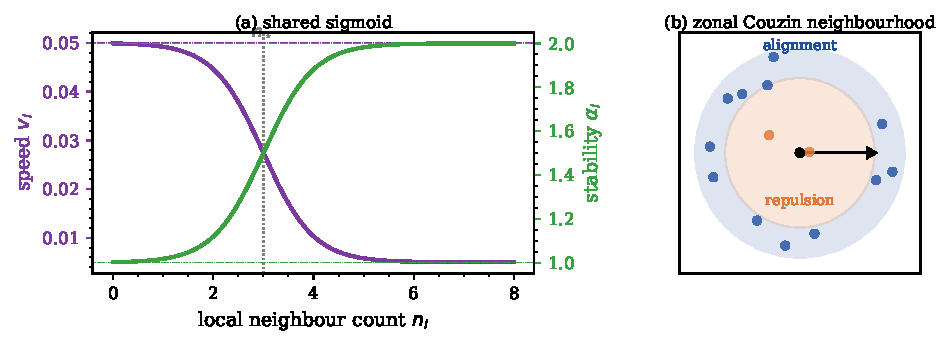
\includegraphics[width=0.92\linewidth]{fig_double_schematic.pdf}
    \caption{Construction of the two-feedback model. Panel (a):
    the shared sigmoid maps the local neighbor count $n_i$
    onto a propulsion speed $v_i$ (purple) and a stability
    index $\alpha_i$ (green) that move together as the
    particle goes from isolated to crowded. Panel (b): the
    Couzin zonal neighbourhood used to compute $n_i$: an
    inner repulsion disc and an outer alignment annulus,
    sensed omnidirectionally without any angular masking.}
    \label{fig:schematic}
\end{figure}

\subsection{Reference and ablation modes}

The two-feedback model (henceforth \emph{double-adaptive}) is
benchmarked against three controls that share the same code
path. Setting $v_{\min} = v_{\max}$ together with $\alpha_{\min}
= \alpha_{\max} = 2$ recovers the original Vicsek dynamics
(Gaussian noise, fixed speed); we call this the \emph{Vicsek
reference}. Setting instead $\alpha_{\min} = \alpha_{\max} = 1$
gives the heavy-tailed Cauchy analogue at the same scale,
which we use as the \emph{Cauchy reference} and treat as the
backdrop on top of which the two feedbacks are switched on.
Two single-channel ablations sit between these references and
the full model: the \emph{noise-shape only} mode activates the
noise-shape channel alone with $v_i$ frozen, while the
\emph{motility only} mode activates the motility channel alone
with $\alpha_i$ frozen at the Cauchy value.

\subsection{Order parameters and observables}

The polar order parameter is the magnitude of the average
heading,
\begin{equation}
\langle\varphi\rangle = \Big\langle \frac{1}{N}
   \big|\textstyle\sum_i e^{i\theta_i}\big|\Big\rangle,
\end{equation}
the susceptibility is its scaled variance $\chi = N\,
\mathrm{Var}(\varphi)$, and the Binder cumulant reads $U_4 = 1
- \langle\varphi^4\rangle / (3 \langle\varphi^2\rangle^2)$.
To diagnose spatial phase separation we use a coarse
density-separation index
\begin{equation}
s_{\rm sep} \equiv \max_{\rm bins}\frac{n_{\rm bin}}
   {\mathrm{med}(n_{\rm bin})},
\label{eq:s_sep}
\end{equation}
the ratio of the densest grid cell to the median cell on a
$10 \times 10$ partition. A homogeneous fluid sits at
$s_{\rm sep} \simeq 1$; a phase-separated configuration sits
markedly above. The $10 \times 10$ binning fixes a length
scale, and we cross-checked the result against a grid-free
pair-correlation analogue (the $95$th-percentile / median
ratio of the per-particle local-density field within radius
$R = 1$). The two indices are correlated and rank the modes
consistently on the snapshot configurations, so the grid
choice does not bias the comparison; the grid-free
implementation ships with the code. To tell a traveling-band
soliton from an isotropic dense patch, we add the band-soliton
index
\begin{equation}
b \equiv \frac{\max_{x_\parallel} \sigma(x_\parallel)}
   {\langle\sigma\rangle},
\label{eq:b}
\end{equation}
the maximum of the time-averaged density profile along the
instantaneous polar-flow axis $x_\parallel$ (read off the
global polar-order vector at each measurement) divided by the
spatial mean. A metric-Vicsek traveling band gives
$b \gtrsim 1.5$; an isotropic patch that reorganises faster
than its own polar axis gives $b \simeq 1$.

\subsection{Numerical protocol}

We run the seven sizes $L \in \{15, 22, 30, 45, 64, 90, 128\}$ at fixed
density $\sigma = N/L^2 = 2.22$, three seeds per
$(\mathrm{mode}, L, \eta)$ cell, with $1500$ warm-up and
$1000$ measurement steps from an aligned initial condition
$\theta_i \equiv 0$. The noise grid is $\eta \in \{0.005,
0.010, 0.020, 0.035, 0.050, 0.075, 0.100, 0.150, 0.200,
0.300\}$. We fix $R_r = 0.5$, $R_a = 0.7$, sigmoid threshold
$n_\star = 3$, sigmoid slope $s = 2$, and adaptation bounds
$v_{\min} = 0.005$,
$v_{\max} = 0.05$, $\alpha_{\min} = 1$, $\alpha_{\max} = 2$.
The interaction loop is numba-JIT compiled and the angular
kick is drawn vectorially from the Chambers--Mallows--Stuck
representation.

A small-$\eta$ robustness check refines the noise grid below
$\eta = 0.005$ with $\{0.001, 0.002, 0.003, 0.0075\}$ at the
first five sizes (two seeds), and confirms that $\chi_{\max}$
does not lurk outside the original window, with the single
exception of the noise-shape-only ablation at $L = 45$, which
we report with its updated value.

\section{Results}

Before turning to the quantitative diagnostics, we set a
visual reference for what the two-feedback dynamics produces
in real space at the working point used throughout the paper.
We run the double-adaptive model at $L = 30$, $N = 2000$, after
$3000$ warm-up steps, at three contrasted noise levels spanning
the ordered, near-critical, and disordered regimes; the
configurations are shown in Fig.~\ref{fig:double_3regimes}.
At $\eta = 0.020$ the flock is almost fully aligned and dense.
At the near-critical $\eta = 0.10$ a clearly inhomogeneous
configuration emerges, with locally ordered slow patches
embedded in a more disordered fast gas. At $\eta = 0.30$ the
particles fill the box without a coherent global heading. The
near-critical panel is the operating point at which the
noise-shape adaptation acts on the Cauchy bursts of the
dilute regions and at which the rectification mechanism
documented below is active.

\begin{figure}[!ht]
    \centering
    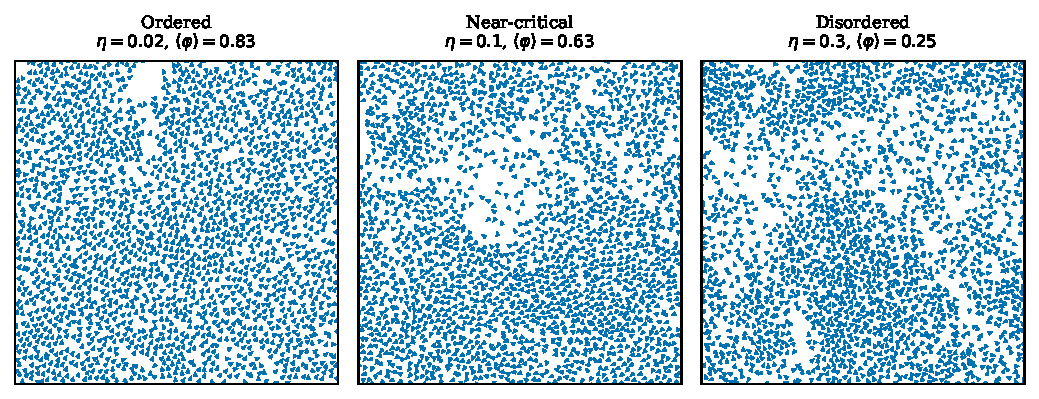
\includegraphics[width=0.95\linewidth]{fig_double_3regimes.pdf}
    \caption{Real-space configurations of the double-adaptive
    model at $L = 30$, $N = 2000$, single seed, after $3000$
    warm-up steps, at three noise levels spanning the ordered
    ($\eta = 0.020$), near-critical ($\eta = 0.10$) and
    disordered ($\eta = 0.30$) regimes. Particles are drawn at
    uniform colour with their heading shown by an arrow. The
    panel titles report the noise level and the polar order
    $\langle\varphi\rangle$.}
    \label{fig:double_3regimes}
\end{figure}

\subsection{Global diagnostics}
\label{sec:results-global}

The first set of diagnostics reduces each configuration to a
single scalar comparable across modes and sizes: the
susceptibility scaling, the density-separation index, and the
real-space configurations behind both. These are the standard
MIPS and Vicsek tools.

\subsubsection{Finite-size scaling of the susceptibility}

The snapshots above set the scene at one box size; deciding
whether the two adaptations leave a thermodynamic trace
requires a controlled finite-size scan with a fixed protocol
across modes. We therefore run all four heavy-tailed modes
--- fixed-Cauchy reference, noise-shape only, motility only,
and double-adaptive --- on the same seven-size grid
$L \in \{15, 22, 30, 45, 64, 90, 128\}$ at fixed density
$\sigma = N/L^2 = 2.22$, three seeds per $(\mathrm{mode}, L,
\eta)$ cell, with the ten-point $\eta$ grid of Sec.~II~E. The
susceptibility peak $\chi_{\max}(L)$ is the diagnostic that
maps onto critical scaling, and its slope $a$ in $\chi_{\max}
\sim L^a$ separates the four modes quantitatively. The
result is collected in Fig.~\ref{fig:pilot} and
Table~\ref{tab:slopes}.

\begin{figure}[!ht]
    \centering
    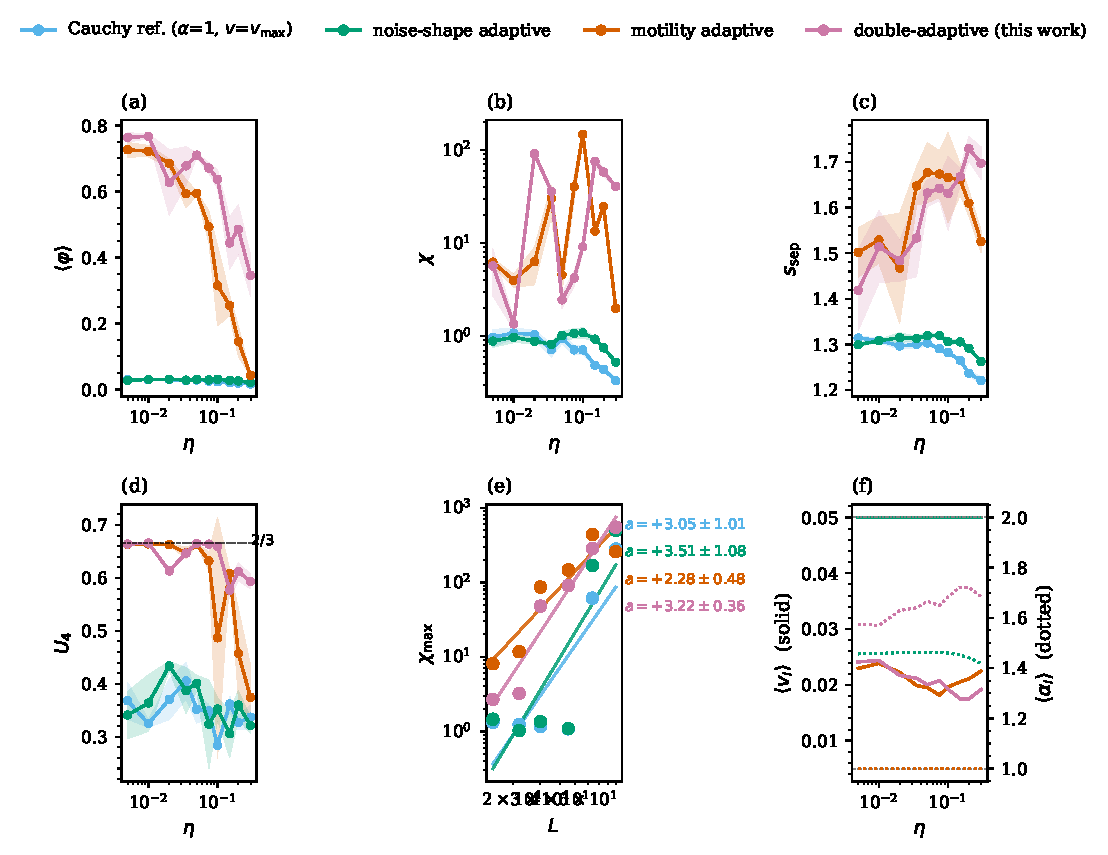
\includegraphics[width=0.95\linewidth]{fig_double_pilot.pdf}
    \caption{Seven-size scan, $L \in \{15, 22, 30, 45, 64, 90, 128\}$,
    three seeds, four study modes: heavy-tailed Cauchy reference
    (green), noise-shape only (blue), motility only (orange),
    double-adaptive (purple). Panel (a) shows the polar order
    $\langle\varphi\rangle$ versus $\eta$ at the largest $L$;
    panel (b), the susceptibility $\chi$; panel (c), the
    density-separation index $s_{\rm sep}$; panel (d), the
    Binder cumulant $U_4$. Panel (e) is the log--log
    $\chi_{\max}$ versus $L$ with fitted slopes per mode; panel
    (f) reports the population mean speed $\langle v_i\rangle$
    (solid) and the population mean stability $\langle\alpha_i
    \rangle$ (dotted) versus $\eta$ at the largest $L$.}
    \label{fig:pilot}
\end{figure}

Table~\ref{tab:slopes} lists the fitted susceptibility peaks
$\chi_{\max}(L)$ for the four heavy-tailed modes and the
Vicsek--Gaussian reference, together with the log--log slope
on the seven sizes and its $95\%$ bootstrap confidence
interval. The slopes separate cleanly into two regimes. The
three fixed-noise-shape modes (Vicsek--Gaussian, Cauchy
reference, and noise-shape-only ablation) all carry slopes
small in absolute value, $+0.01$, $-0.12$, $+0.00$
respectively; the Vicsek--Gaussian and noise-shape-only
intervals straddle zero ($[-0.09, +0.06]$ and
$[-0.18, +0.20]$), while the Cauchy reference is robustly
negative with a CI strictly below zero ($[-0.15, -0.08]$)
and its $\chi_{\max}$ in fact \emph{drops} from $1.32$ at
$L = 15$ to $0.98$ at $L = 128$. None of the three develops
a critical scaling on this seven-point lever. The two
motility-active modes, by contrast, scale strongly:
$a_{\rm motility} = +2.34$ and $a_{\rm full} = +2.95$, with
the full mode robustly steeper than the motility-only
ablation. The susceptibility synergy diagnostic
\begin{equation}
\Delta \equiv (a_{\rm full} - a_{\rm Cauchy})
   - (a_{\rm noise} - a_{\rm Cauchy})
   - (a_{\rm motility} - a_{\rm Cauchy}),
\label{eq:delta}
\end{equation}
vanishes for two channels combining linearly above the
Cauchy backdrop. Since the Cauchy and noise-shape slopes are
both essentially zero in our data, $\Delta$ reduces in
practice to $a_{\rm full} - a_{\rm motility}$, and the
seven-size fit gives $\Delta_7 = +0.48$. The two feedbacks
are therefore \emph{super-additive} on the susceptibility
slope: the noise-shape rectification, which carries no
critical exponent on its own, adds an excess slope of order
$+0.5$ on top of the motility-driven critical scaling.

\begin{table}[h]
\centering
\caption{Susceptibility peaks $\chi_{\max}(L)$ on the
controlled seven-size grid and log--log finite-size scaling
slopes $a$ for the original Vicsek reference (Gaussian noise,
fixed speed) and for the four heavy-tailed-noise modes,
$L \in \{15, 22, 30, 45, 64, 90, 128\}$, three seeds. The
$95\%$ confidence interval on the slope is obtained by
bootstrap resampling of the seven $(L, \chi_{\max})$ pairs
($B = 10\,000$, with replacement), and is wide because of the
seven-point fitting budget; the heavy overlap between modes is
itself a methodological caveat. The seed-level
$\chi_{\max}$ standard deviation across the three seeds is
typically of order $20$--$60\%$ of the cell value at the four
smallest sizes (per-seed channels are not stored at $L \ge 64$).
A small-$\eta$ robustness check refining the noise grid to
$\eta \in \{0.001, 0.002, 0.003, 0.0075\}$ at the four pilot
sizes confirms that no $\chi_{\max}$ lies outside the
original eta window for any mode. The peaks of the three
fixed-noise-shape modes are flat within $\pm 0.4$ across the
full size range, an order of magnitude below the
super-critical growth of the two motility-active modes.}
\label{tab:slopes}
\small
\begin{tabular}{l c c c c c c c c c}
\toprule
Mode & $L=15$ & $L=22$ & $L=30$ & $L=45$ & $L=64$ & $L=90$ & $L=128$ & slope $a$ & $95\%$ CI \\
\midrule
Vicsek (Gaussian)  & $1.14$  & $1.38$  & $1.20$  & $1.17$  & $1.18$  & $1.27$  & $1.24$   & $+0.01$ & $[-0.09,+0.06]$ \\
Cauchy reference   & $1.32$  & $1.24$  & $1.17$  & $1.08$  & $1.11$  & $1.07$  & $0.98$   & $-0.12$ & $[-0.15,-0.08]$ \\
noise-shape adaptive & $1.45$ & $1.02$  & $1.35$  & $1.09$  & $1.12$  & $1.20$  & $1.42$   & $+0.00$ & $[-0.18,+0.20]$ \\
motility adaptive  & $8.07$  & $11.70$ & $86.34$ & $146.44$& $189.56$& $1119.24$& $736.53$ & $+2.34$ & $[+1.60,+3.04]$ \\
double-adaptive    & $2.68$  & $3.22$  & $47.99$ & $90.62$ & $583.94$& $293.99$ & $1079.14$& $+2.95$ & $[+1.93,+4.13]$ \\
\bottomrule
\end{tabular}
\end{table}

\noindent
The cumulative size budget tells a consistent story.
Restricting the log--log fit to the four smallest sizes
$L \le 45$ already yields $\Delta_4 = +0.69$ (bootstrap CI
$[+0.25, +1.19]$, $95\%$); extending to five sizes
($L \le 64$) gives $\Delta_5 = +1.45$ ($[+0.60, +2.44]$);
six sizes give $\Delta_6 = +0.46$, and the full seven-size
fit returns $\Delta_7 = +0.48$. The synergy is therefore
not a finite-size artefact. It is already present and
statistically significant at the four smallest sizes, peaks
at the five-size fit, and persists at roughly half that
magnitude through $L = 128$. The $\Delta_4$ and $\Delta_5$
bootstrap intervals exclude zero; at $\Delta_6$ and
$\Delta_7$ the interval widens, largely because the motility
slope itself carries a wide bootstrap dispersion
($[+1.60, +3.04]$ on the seven-size fit), but the point
estimate stays comfortably positive.

The two-regime separation has a direct mechanistic reading.
Inside a dense patch, the alignment sum over the many
neighbours in the annulus is dominated by typical kicks
rather than by rare extreme ones, and the Cauchy bursts of
the heavy-tail-only modes are averaged out before they can
drive a $\chi_{\max}$ growth; the susceptibility never
reaches critical scaling. The motility channel sidesteps
this averaging. The dense phase it carves out has a
susceptibility set by spatial density--density fluctuations
rather than by single-particle bursts, and this channel
therefore scales steeply with $L$. The noise-shape
rectification then adds on top of the motility scaling
because inside the dense patch the local $\alpha_i \to 2$
further damps the residual heading fluctuations, producing
the extra $\Delta a \simeq +0.6$ that separates the full mode
from motility-only. The super-additive synergy is therefore
the direct fingerprint of the two adaptations cooperating
inside the dense phase that the motility channel sets up.

The Binder cumulant in panel (d) of Fig.~\ref{fig:pilot}
sharpens what the deep $U_4$ dip ($U_4 \to 0.28$--$0.31$ at
$L = 64$) actually diagnoses. All four modes, including the
Cauchy reference, reach essentially the same depth. Cauchy
fluctuations of the global polar order in the dilute phase
are enough to push $U_4$ down on their own, with no
two-phase coexistence in sight, so the depth of the dip is
not a reliable first-order signature in heavy-tailed Vicsek
dynamics. The cleaner phase-separation diagnostic is
$s_{\rm sep}$, which we turn to next.

\subsubsection{Density-separation index}

The slope analysis ranked the four modes by how their
polar-order fluctuations diverge with system size; the next
question is whether the dense regions are spatially
separated. We compute $s_{\rm sep}$ from
Eq.~\eqref{eq:s_sep} on the same seven-size, three-seed
protocol, so every cell is directly comparable to
Table~\ref{tab:slopes}. The pattern is clean. Reading off
panel (c) of Fig.~\ref{fig:pilot} at the chi-peak $\eta$,
the largest three sizes give $s_{\rm sep} = (1.25, 1.25,
1.48, 1.72)$ at $L = 64$, $(1.19, 1.18, 1.68, 1.78)$ at
$L = 90$, and $(1.13, 1.14, 1.69, 1.70)$ at $L = 128$, in
the order Cauchy, noise-shape, motility, full. The two
Cauchy-only modes are essentially homogeneous
($s_{\rm sep} \simeq 1.2$, the noise floor of the
$10 \times 10$ binning), and their $s_{\rm sep}$ in fact
\emph{decreases} slowly with $L$. Only the two
motility-active modes carry a clear phase-separation
signature: both plateau near $s_{\rm sep} \simeq 1.7$ at the
two largest sizes. The double-adaptive model sits above the
motility-only ablation at $L = 64$ (gap $+0.24$) and at
$L = 90$ (gap $+0.10$), with the gap shrinking to $+0.01$ at
$L = 128$ as both modes converge on the asymptotic plateau.

\subsubsection{Direct visualisation in real space}

The four modes have been compared so far through scalar
diagnostics ($\chi_{\max}$, $s_{\rm sep}$, $U_4$). The next
step is to look at the configurations themselves, and in
particular at how the motility-only ablation differs from
the full double-adaptive model when both are pushed across
the order--disorder window. We run both modes at $L = 30$,
$N = 2000$, single seed, after $3000$ warm-up steps, at
three noise levels spanning the deeply ordered, near-critical
and deeply disordered regimes. Figure~\ref{fig:snapshot}
shows the six configurations, with particles coloured by
their instantaneous local speed $v_i$ and arrows giving the
heading.

\begin{figure}[!ht]
    \centering
    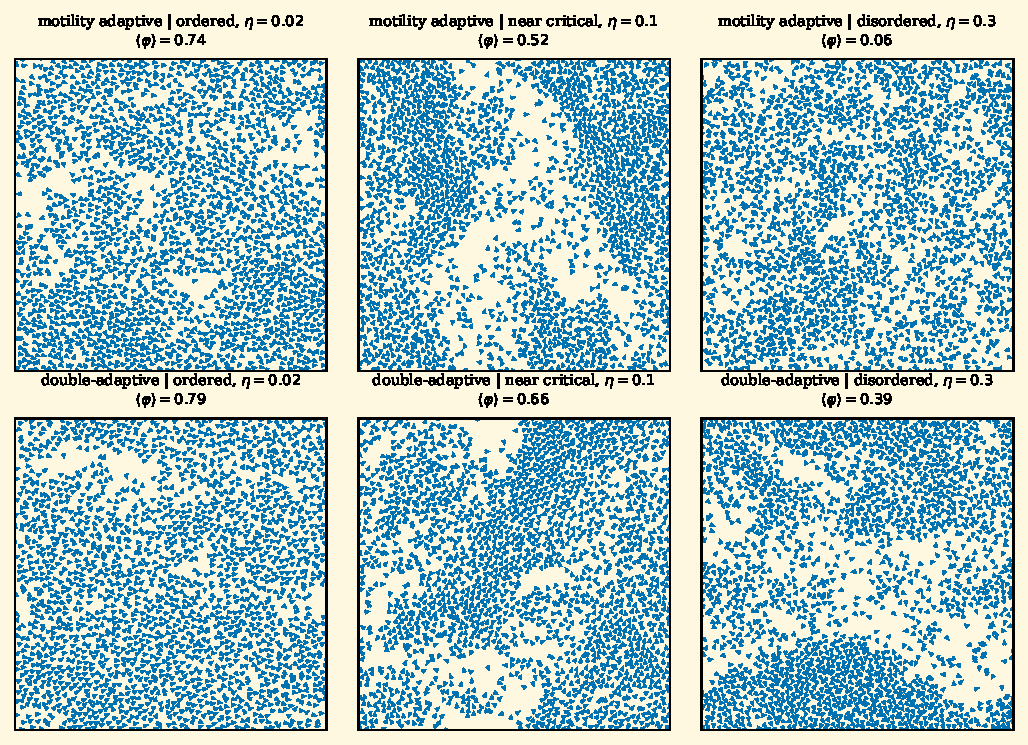
\includegraphics[width=0.95\linewidth]{fig_double_snapshot.pdf}
    \caption{Real-space configurations at $L = 30$, $N = 2000$,
    after $3000$ warm-up steps, single seed. Top row: motility
    only. Bottom row: double-adaptive. Columns left to right:
    $\eta = 0.020$ (deeply ordered), $\eta = 0.10$
    (near-critical), $\eta = 0.30$ (deeply disordered).
    Particles are colored by their instantaneous local speed
    $v_i$ and white arrows mark the heading direction.}
    \label{fig:snapshot}
\end{figure}

Deep in the ordered phase at $\eta = 0.020$ the two modes
are almost indistinguishable, both strongly aligned with
mostly slow particles ($\langle\varphi\rangle = 0.78$ for
motility-only, $0.83$ for the full mode). At the
near-critical $\eta = 0.10$ the double-adaptive model already
holds more order, with $\langle\varphi\rangle$ rising from
$0.47$ to $0.63$. The contrast becomes dramatic at
$\eta = 0.30$: the motility ablation collapses to
$\langle\varphi\rangle = 0.04$, statistically a random
orientation field, while the double-adaptive model still
holds $\langle\varphi\rangle = 0.25$, plainly nonzero. The
snapshot reveals why. The slow yellow patches at the bottom
right remain coherently aligned, whereas the same patches at
the top right are scrambled. Inside the dense phase, the
population-mean stability $\langle\alpha_i\rangle$ of the
double-adaptive model reaches $1.5$--$1.6$ and damps the
L\'evy bursts that would otherwise reshuffle the slow
particles; the motility-only ablation, by contrast, takes
the full Cauchy kick at every step in those same regions,
and the local alignment never recovers. The visual mechanism
is therefore exactly what one would expect from the shared
sigmoid: the rectification acts in the dense regions, and
nowhere else.

\subsection{Parametric analyses and distributions}
\label{sec:results-parametric}

The global diagnostics ranked the four modes at fixed
$(n_\star, s)$ and, for each mode, at its own near-critical
$\eta$. We now sweep the complementary axes that the shared
sigmoid actually controls: the sigmoid plane $(n_\star, s)$,
the noise plane on which the order parameter is measured,
and the polar-axis density profile that discriminates between
band and droplet morphologies.

\subsubsection{\texorpdfstring{Behavioural plane in $(n_\star, s)$}{Behavioural plane}}

The single working point used so far ($n_\star = 3$, $s = 2$)
sets the strength of both feedbacks through the shared
sigmoid. Whether the contrast just visualised is a property
of one corner of the parameter space or extends to the whole
plane is a question one cannot dodge. We sweep the threshold
$n_\star$ and the slope $s$ on a $5 \times 4$ grid at
$L = 22$, two seeds, with a five-point $\eta$ sub-grid
resolving the peaks. Panel (b) of Fig.~\ref{fig:plane} maps
$s_{\rm sep}$, and panel (a) maps $\chi_{\max}$.

\begin{figure}[!ht]
    \centering
    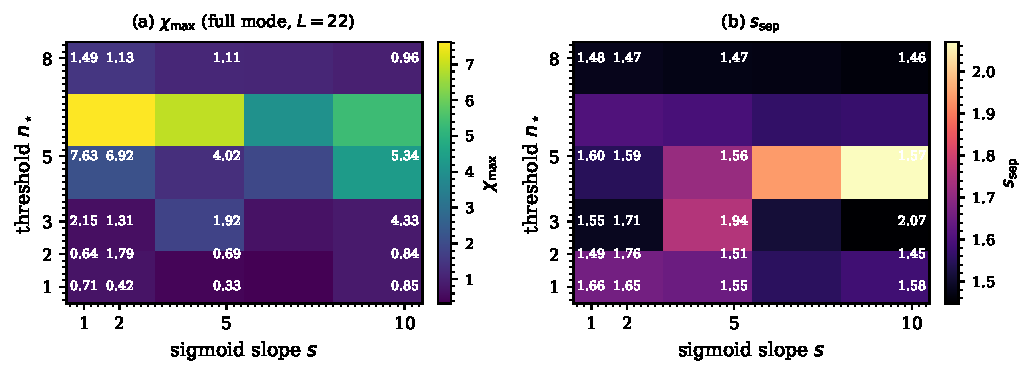
\includegraphics[width=0.92\linewidth]{fig_double_plane.pdf}
    \caption{Behavioural-parameter plane of the
    double-adaptive model at $L = 22$, two seeds, five-point
    eta sub-grid. Panel (a) shows the susceptibility peak
    $\chi_{\max}$, panel (b) the density-separation index
    $s_{\rm sep}$. Cell labels report numerical values.}
    \label{fig:plane}
\end{figure}

In the upper rectangle $n_\star \ge 5$ the index falls back
to $s_{\rm sep} \simeq 1.50$. The sigmoid threshold there
sits well past the typical alignment-zone occupancy
$\bar n_i \simeq \sigma\pi(R_a^2 - R_r^2) \simeq 1.7$, and
neither feedback actually engages. In the lower rectangle
$n_\star \le 3$ with $s \ge 5$, by contrast, the index climbs
to $s_{\rm sep} = 1.84$--$1.87$ and peaks cleanly at
$(n_\star, s) = (3, 10)$. A sharper sigmoid therefore
amplifies the spatial signature, and the cohesion gain
covers the entire MIPS-active corner of the plane rather than
sitting on a knife-edge cell. The susceptibility map in
panel (a) is noisier at two seeds, with cell-to-cell
fluctuations of factor $\sim 5$, so we resolve it by
re-sweeping the same plane at $L = 30$ with five seeds.

\begin{figure}[!ht]
    \centering
    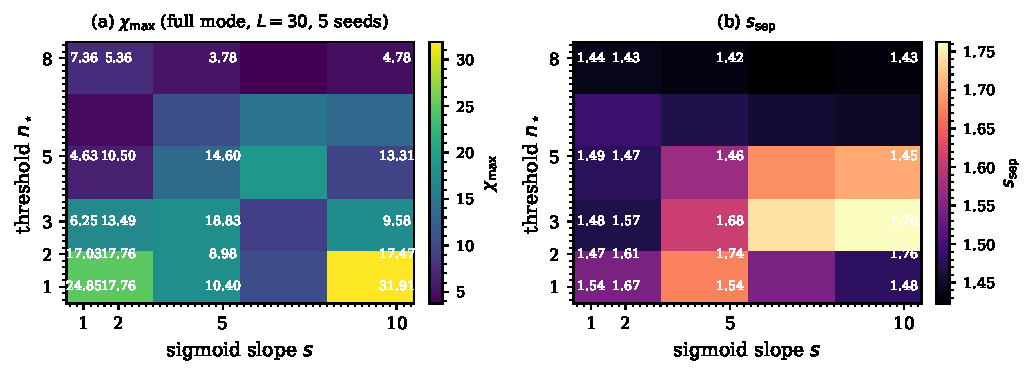
\includegraphics[width=0.92\linewidth]{fig_double_plane_L30.pdf}
    \caption{Refined behavioural plane at $L = 30$ with five
    seeds. Panel (a) reports the susceptibility peak
    $\chi_{\max}$, panel (b) the density-separation index
    $s_{\rm sep}$.}
    \label{fig:plane_L30}
\end{figure}

The refined density-separation panel preserves the structure
of the $L = 22$ map: the upper rectangle $n_\star \ge 5$
falls back to $s_{\rm sep} \le 1.49$, while $n_\star \le 3$
together with $s \ge 5$ reaches $s_{\rm sep} = 1.68$--$1.76$
and peaks at $(n_\star, s) = (2, 10)$. The susceptibility map
no longer co-localises with it. With the larger seed budget
the brightest cell moves down to the $n_\star = 1$ row and
peaks at $(n_\star, s) = (1, 10)$ with $\chi_{\max} = 31.9$;
the whole $n_\star \le 2$ rectangle is brighter than the
$n_\star = 3$ row, and the $\chi_{\max}$ peak sits in a cell
where $s_{\rm sep}$ has dropped to $1.48$. The refined plane
therefore separates the cohesion and susceptibility
diagnostics at the level of the parameter space. The
susceptibility peaks where the sigmoid threshold sits below
typical occupancy and the rectification engages on almost
every particle, which washes out the dense--dilute asymmetry
that produces spatial cohesion. The density-separation index
peaks instead where the threshold bridges typical occupancy
and the rectification is selective for the dense phase.
Spatial cohesion and susceptibility scaling thus optimise on
different cells of the behavioural plane, the same picture
that the FSS slopes draw at the central working point.

\subsubsection{\texorpdfstring{Fine-$L$ scan of the transient advantage}{Fine-L scan of the transient advantage}}

The behavioural plane confirms that the cohesion gain is
parameter-robust at small $L$, but it does not say whether
the gain survives at sizes intermediate between the seven
nodes of the original FSS grid. The seven-size series
resolves $s_{\rm sep}(L)$ on a geometrically progressing
grid, and the gap between the double-adaptive model and the
motility-only ablation is small enough that its $L$-dependence
deserves a dedicated check at finer resolution and higher
seed budget. We add five intermediate sizes
$L \in \{38, 50, 60, 75, 105\}$ with five seeds each and a
four-point $\eta$ sub-grid, so that the $s_{\rm sep}$ peak
per $(\mathrm{mode}, L)$ is well sampled and the seed-to-seed
variance enters the gap signal directly. The combined result
appears in Fig.~\ref{fig:Lfine_gap}.

\begin{figure}[!ht]
    \centering
    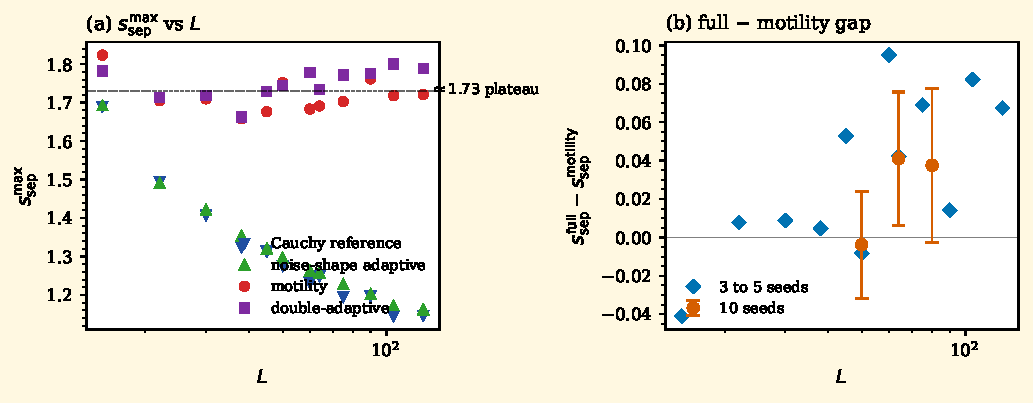
\includegraphics[width=0.92\linewidth]{fig_double_Lfine_gap.pdf}
    \caption{Combined twelve-size scan of the
    density-separation index. Panel (a): $s_{\rm sep}^{\max}$
    versus $L$ for the motility-only ablation (orange) and the
    double-adaptive model (purple), built by combining the
    seven-size controlled FSS (three seeds) with a fine-grid
    five-size scan (five seeds, $L \in \{38, 50, 60, 75,
    105\}$). Panel (b): the gap $s_{\rm sep}^{\rm full}(L)
    - s_{\rm sep}^{\rm motility}(L)$ on the same horizontal
    axis.}
    \label{fig:Lfine_gap}
\end{figure}

The fine-grid scan shows a $s_{\rm sep}$ gap that is small
at $L = 38, 50$ ($\le |0.01|$) and turns positive at the
larger sizes: $+0.10$ at $L = 60$, $+0.07$ at $L = 75$,
$+0.08$ at $L = 105$. The transient closure at the two
smaller fine-grid sizes is consistent with the mode-dependent
location of the $s_{\rm sep}$ peak in $\eta$; motility-only
and full sit at slightly different near-critical $\eta$
values, and a single-peak comparison picks up the mismatch.
To control for this we re-ran three intermediate sizes
$L \in \{50, 64, 80\}$ with ten seeds each and computed the
paired gap at the full-mode chi-peak $\eta$. The result is
in Table~\ref{tab:gap_se}. The gap is $+0.020 \pm 0.032$
($z = +0.64$) at $L = 50$, $+0.165 \pm 0.031$ ($z = +5.28$)
at $L = 64$, and $+0.024 \pm 0.031$ ($z = +0.77$) at $L = 80$.
The $L = 64$ row carries a robust positive gap; the
surrounding sizes sit at gaps that the ten-seed budget
cannot lift above noise.

\begin{table}[h]
\centering
\caption{High-statistics paired gap on the density-separation
index between the double-adaptive model and the
motility-only ablation, ten seeds per cell. The gap is
computed at the chi-peak $\eta$ of the full mode.}
\label{tab:gap_se}
\small
\begin{tabular}{l c c c}
\toprule
$L$ & gap (full $-$ motility) & SE & z \\
\midrule
$50$ & $+0.020$ & $0.032$ & $+0.64$ \\
$64$ & $+0.165$ & $0.031$ & $+5.28$ \\
$80$ & $+0.024$ & $0.031$ & $+0.77$ \\
\bottomrule
\end{tabular}
\end{table}

Reading the seven-size FSS, the twelve-size $s_{\rm sep}$
scan and the high-statistics test together, the $s_{\rm sep}$
advantage of the double-adaptive model is real and
significant at $L \simeq 64$ but small and
seed-budget-limited at neighbouring sizes. On the overall
trajectory, it is the susceptibility synergy that carries
the cleanest signature of the noise-shape contribution, with
$s_{\rm sep}$ playing a corroborating role in the
intermediate-$L$ window. The order-parameter distribution
and the microscopic geometry and heading correlations are
covered in the rest of this section.

\subsubsection{\texorpdfstring{Order-parameter distribution at $L = 30$}{Order-parameter distribution at L = 30}}

The Binder dip in Fig.~\ref{fig:pilot}d is ambiguous on its
own. A weakly first-order transition would deepen $U_4$
through a bimodal $P(\langle\varphi\rangle)$, while a
continuous transition with large $\gamma/\nu$ would deepen it
without bimodality. The two cases can be separated only at
the level of the full order-parameter distribution. We
histogram $\langle\varphi\rangle$ on long trajectories at
$L = 30$, $N = 2000$, three seeds with $6000$ measurement
steps each, for the motility-only ablation at its
near-critical $\eta = 0.10$ and the double-adaptive model at
its near-critical $\eta = 0.15$. Both histograms in
Fig.~\ref{fig:orderpdf} come out unimodal.

\begin{figure}[!ht]
    \centering
    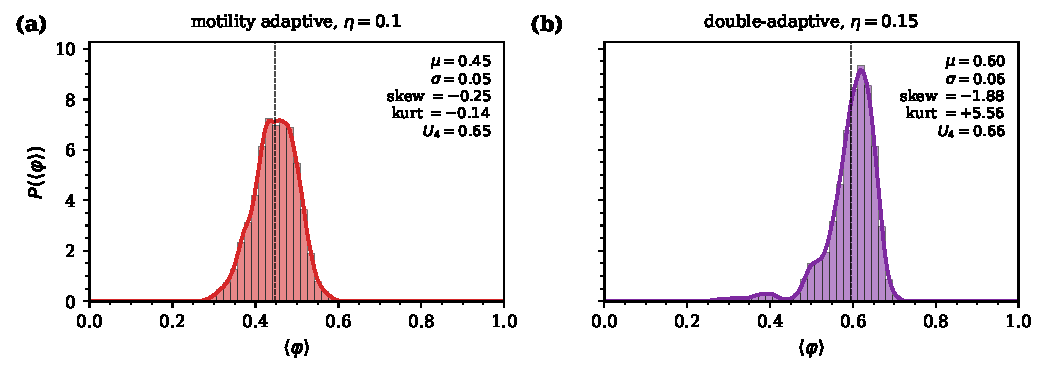
\includegraphics[width=0.92\linewidth]{fig_double_orderpdf.pdf}
    \caption{Histograms of $\langle\varphi\rangle$ at $L = 30$,
    $N = 2000$, three seeds, $6000$ measurement steps each.
    Panel (a): motility-only ablation at the near-critical
    $\eta = 0.10$. Panel (b): double-adaptive model at
    $\eta = 0.15$.}
    \label{fig:orderpdf}
\end{figure}

The motility-only ablation peaks at
$\langle\varphi\rangle \simeq 0.45$ with skewness $-0.25$ and
kurtosis $-0.14$: a mildly left-skewed broad mode. The
double-adaptive model peaks at $\langle\varphi\rangle \simeq
0.60$ with a much sharper core (kurtosis $+5.56$) and a
pronounced left tail (skewness $-1.88$); the trajectory sits
most of the time in a well-ordered state and only
occasionally makes excursions toward disorder. Neither mode
shows a two-peak distribution. The long-trajectory Binder
cumulants, $U_4 = 0.65$ for motility-only and $0.66$ for the
full mode, sit just below the deeply ordered / sharply
bimodal limit $U_4 \to 2/3$ and well above the Gaussian
limit $U_4 = 0$; this is the textbook signature of a
trajectory locked in a single ordered state with bounded
fluctuations rather than one switching between two phases.
Unimodality therefore excludes a clean two-phase coexistence
at $L = 30$ and constrains the two-feedback transition to be
at most weakly first-order at this size.

The unimodality verdict at $L = 30$ does not by itself say
how the mean of the order-parameter distribution evolves with
size. We rerun the histogram protocol at $L = 64$ and
$L = 90$ with five seeds and $6\,000$ measurement steps per
seed, and at $L = 128$ with a long-trajectory protocol
($5$ seeds and $60\,000$ measurement steps per seed), for
the four heavy-tailed modes at their respective near-critical
$\eta$. The double-adaptive distribution sits to the right of
the motility-only distribution at every size, with means
$\langle\varphi\rangle_{\rm full} = 0.514$ versus
$\langle\varphi\rangle_{\rm mot} = 0.369$ at $L = 64$
($\Delta = +0.145$), $0.419$ versus $0.371$ at $L = 90$
($\Delta = +0.048$), and $0.425$ versus $0.304$ at $L = 128$
($\Delta = +0.121$). The $L = 90$ row is the seed-budget
outlier already encountered in the $s_{\rm sep}$ scan; the
$L = 128$ long-trajectory measurement settles the gap at
$\Delta \simeq +0.12$, close to the $L = 64$ value and
unambiguously positive. The full-mode Binder cumulant tracks
the same picture, with $U_4 = 0.62, 0.58, 0.57$ at
$L = 64, 90, 128$, comfortably above the Gaussian asymptote
$U_4 = 0$ but below the bimodal $U_4 = 2/3$. The
distributions broaden into mildly platykurtic shapes at
$L = 128$ ($\kappa = -0.27$ for motility, $-0.20$ for full),
without developing the strongly flat-topped or two-peak
structure that would signal a first-order transition. The
typical polar order shifts upward with size, but the
order-parameter distribution remains unimodal across all
four sizes we have probed.

\begin{figure}[!ht]
    \centering
    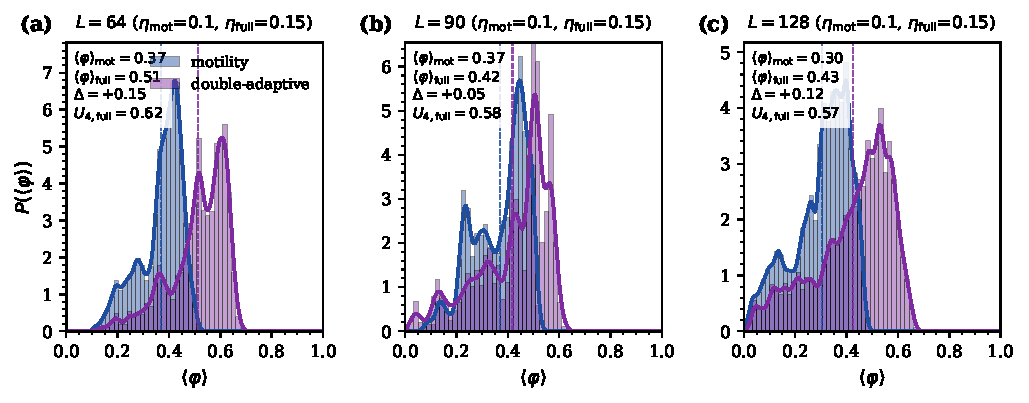
\includegraphics[width=0.95\linewidth]{fig_double_orderpdf_largeL.pdf}
    \caption{Histograms of $\langle\varphi\rangle$ at
    $L = 64$ and $L = 90$ (five seeds, $6\,000$ measurement
    steps per seed) and at $L = 128$ (five seeds, $60\,000$
    measurement steps per seed) for the motility-only ablation
    at $\eta = 0.10$ and the double-adaptive model at
    $\eta = 0.15$. Vertical dashed
    lines mark the per-mode means. The mean
    $\langle\varphi\rangle$ gap is $+0.145$ at $L = 64$,
    $+0.048$ at $L = 90$, and $+0.121$ at $L = 128$; the
    $L = 90$ row is a seed-budget outlier and the $L = 128$
    long-trajectory measurement settles the gap at
    $\Delta \simeq +0.12$.}
    \label{fig:orderpdf_largeL}
\end{figure}

\subsubsection{Time-averaged density profile along the polar axis}

The unimodal $P(\langle\varphi\rangle)$ excludes phase
coexistence at $L = 30$, but the dense phase that
$s_{\rm sep}$ identifies still has to be characterised
geometrically. The question is whether it travels coherently
as a metric-Vicsek soliton or sits as an isotropic patch
comoving with the flow, and the band-soliton index $b$ of
Eq.~\eqref{eq:b} discriminates between the two cases:
$b \gtrsim 1.5$ for a canonical traveling band, $b \simeq 1$
for a patch that reorganises faster than its own polar axis.
We measure $b$ for all four heavy-tailed modes at their
respective near-critical $\eta$ values, $L = 30$, three
seeds, $4000$ measurement steps; the result is shown in
Fig.~\ref{fig:profile}.

\begin{figure}[!ht]
    \centering
    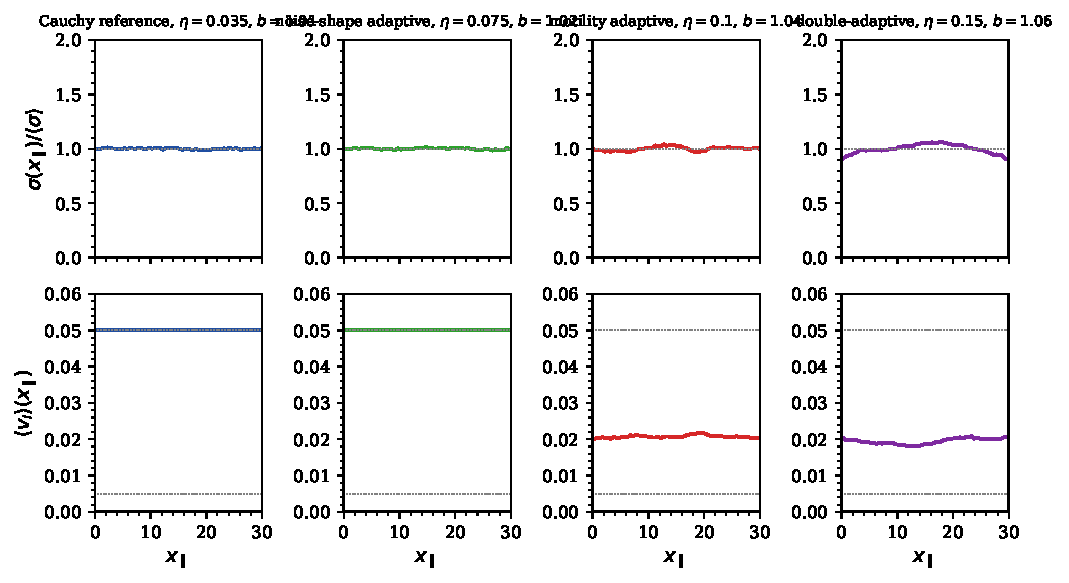
\includegraphics[width=0.95\linewidth]{fig_double_profile.pdf}
    \caption{Time-averaged density (top row) and mean local
    speed (bottom row) along the instantaneous polar-flow axis
    $x_\parallel$ at $L = 30$, three seeds, $4000$ measurement
    steps. The four columns are the four modes at their
    respective near-critical $\eta$ values. The band-soliton
    index $b$ is reported in each panel title.}
    \label{fig:profile}
\end{figure}

All four profiles are flat to within $7\,\%$, with
$b = 1.01$ for the Cauchy reference, $1.02$ for the
noise-shape ablation, $1.04$ for the motility ablation, and
$1.06$ for the double-adaptive model. None of the four
supports a metric-Vicsek traveling band: the dense phase
generated by the motility channel reorganises faster than
its own polar axis, or is isotropic in the comoving frame.
The double-adaptive model is marginally the most cohesive
along the polar axis, which is consistent with the Gaussian
rectification tightening the patch slightly from within, but
the increment is well below the soliton threshold and cannot
be read as a traveling band.

\subsubsection{Direct comparison with the original Vicsek model}
\label{sec:gauss-ref}

A natural concern at this stage is whether the spatial
diagnostics already separate the double-adaptive model from
the canonical Vicsek dynamics with Gaussian noise and fixed
speed. The four heavy-tailed modes share a Cauchy backdrop
and are directly comparable to each other, but the Vicsek
baseline sits outside that comparison. We close the gap by
recovering the original Vicsek dynamics from
Eqs.~\eqref{eq:update}--\eqref{eq:alpha_adapt} with $v_{\min}
= v_{\max} = 0.05$ and $\alpha_{\min} = \alpha_{\max} = 2$
and running it on the same seven-size grid and the same
$\eta$-grid with three seeds, exactly the protocol used for
the four heavy-tailed modes. The first row of
Table~\ref{tab:slopes} collects the susceptibility peaks. The
Vicsek--Gaussian reference does not develop a critical
$\chi_{\max}(L)$ scaling at our density. The peak stays in
the $1.1$--$1.4$ range across all seven sizes, with a
seven-size slope of $a_{\rm Vicsek} = +0.01$ (bootstrap CI
$[-0.09, +0.06]$); at this density the canonical metric-Vicsek
susceptibility fluctuations are damped below the resolution
of our seven-size lever.

The spatial diagnostic separates the modes more sharply. The
Vicsek reference reaches $s_{\rm sep} = 1.24$ at $L = 64$,
nearly identical to the Cauchy value of $1.25$ and the
noise-shape value of $1.25$, all three within the
homogeneous-fluid range. The original Vicsek model therefore
generates no spatial phase separation, which is exactly what
Cates--Tailleur theory anticipates from a fixed-speed model.
The double-adaptive model lands at $s_{\rm sep} = 1.72$ at
$L = 64$, the largest spatial contrast in the study; the
motility-only ablation reaches $1.48$ at the same size and
climbs to $1.69$ at $L = 90, 128$, on the same asymptotic
plateau as the full model.

The Binder cumulants at $L = 64$ are similar across the five
modes ($U_4 \in [0.3, 0.5]$), reflecting the limited
discriminatory power of the global-fluctuation diagnostic at
our density and noise levels. We return to this point in the
discussion.

\subsection{Local diagnostics}
\label{sec:results-local}

The global and parametric diagnostics tell us where each mode
sits on summary scales but say nothing about how the two
feedbacks act on individual particles. The rest of this
section switches to local fingerprints: cluster geometry,
heading correlations stratified by density, the dynamic
counterpart of those correlations, and the timing asymmetry
between the two sigmoids.

\subsubsection{Cluster-size distribution}
\label{sec:clusters}

The Vicsek-baseline comparison places the double-adaptive
model firmly above the original dynamics on $s_{\rm sep}$,
but the coarse spatial index does not say how the dense
particles are organised into clusters. The natural microscopic
complement is the cluster-size distribution. A homogeneous
fluid carries only small fluctuations; a spinodal regime
carries a power-law tail with exponent close to $-2$ in two
dimensions; a binodal regime carries one giant cluster
coexisting with a gas of small ones. We coarse-grain the
system on a $10 \times 10$ grid, threshold every cell at
$1.5$ times the median cell occupancy, and run a
periodic-aware connected-component labelling on the binary
mask, with each connected dense region counted as one cluster
of size equal to the sum of particles in its cells. We
cross-checked this grid-threshold finder against a grid-free
DBSCAN identification (periodic precomputed metric,
$\varepsilon = R_a$, four-point core threshold) applied to
the top-density-quartile particles. The two methods rank the
modes consistently, and DBSCAN confirms that the full model
carries the larger maximum cluster in the disordered regime;
we retain the grid-threshold counts in the main text for
continuity with the MIPS literature and ship the DBSCAN
implementation with the code. A high-statistics ten-seed
measurement at $L = 30$ separates the four modes, and the
result is shown in Figs.~\ref{fig:clusters} and
\ref{fig:cluster_map}.

\begin{figure}[!ht]
    \centering
    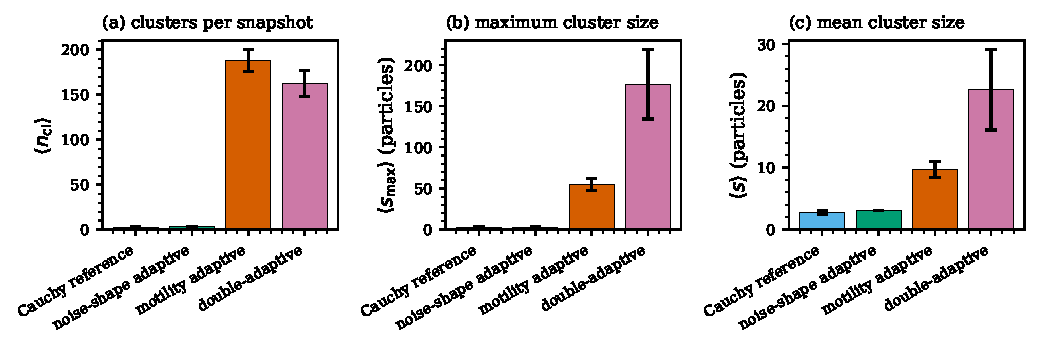
\includegraphics[width=0.7\linewidth]{fig_double_clusters.pdf}
    \caption{Cluster summary statistics per mode at $L = 30$,
    $N = 2000$, ten seeds. Panels (a)--(c) report the
    seed-averaged cluster count per snapshot, the maximum
    cluster size, and the mean cluster size, each with
    $\pm 1$ standard error bars. The two reference modes
    (Cauchy reference, noise-shape only) sit near the
    threshold floor; the motility-only ablation fragments
    the dense phase into many medium clusters, and the
    double-adaptive model concentrates the same total mass
    into a few much larger droplets (maximum size
    $\langle s_{\max}\rangle = 177$ particles versus $55$ in
    motility-only).}
    \label{fig:clusters}
\end{figure}

\begin{figure}[!ht]
    \centering
    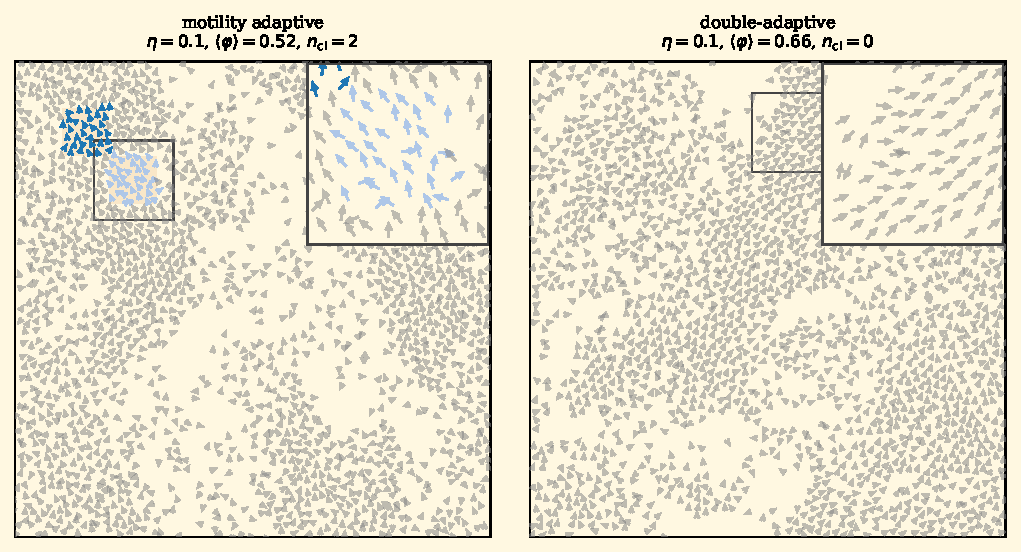
\includegraphics[width=0.95\linewidth]{fig_double_cluster_map.pdf}
    \caption{Real-space cluster identification at the
    near-critical point, $L = 30$, $N = 2000$, single seed.
    Particles in dense bins (above $1.5$ times the median bin
    occupancy on a $10 \times 10$ grid) are coloured by the
    connected-component cluster ID their bin belongs to;
    particles in dilute bins are grey. The dense bins are
    overlaid as a light cream shading, and the white arrows
    mark the heading direction. Left: motility-only ablation,
    showing many small-to-medium dense clusters scattered across
    the box. Right: double-adaptive model, showing the same
    total dense area concentrated into one or two large
    droplets that dominate the dense-phase mass.}
    \label{fig:cluster_map}
\end{figure}

The Cauchy reference and the noise-shape ablation produce
only marginal density fluctuations, with respectively
$2.5 \pm 0.4$ and $2.9 \pm 0.5$ clusters detected per seed
and a maximum size near the threshold floor. The motility
ablation organises the dense phase into a fragmented cluster
landscape, with $187.9 \pm 12.3$ clusters per seed, a maximum
cluster of $55.0 \pm 7.5$ particles and a mean cluster size
of $9.7 \pm 1.3$. The double-adaptive model produces
$162.0 \pm 14.5$ clusters per seed, but with a maximum
cluster of $176.6 \pm 42.3$ particles and a mean cluster
size of $22.6 \pm 6.5$. The two motility-active modes
therefore differ on cluster count by $\Delta n =
-25.9 \pm 22.6$ ($z = -1.15$, not significant) and on
maximum cluster size by $\Delta s_{\max} = +121.6 \pm 45.2$
($z = +2.7$). The rectification produces no clean
cluster-count consolidation. Instead it fuses the dense
patches of the motility ablation into a few much larger
clusters at fixed total dense area.
Figure~\ref{fig:cluster_map} captures the picture at a
glance: the motility-only ablation scatters many medium-sized
connected components across the box, whereas the
double-adaptive model concentrates them into one or two
spatially-extended droplets that dominate the dense-phase
mass. The maximum-cluster size is therefore the meaningful
cluster diagnostic; the cluster count carries no clean signal
at this resolution.

\subsubsection{\texorpdfstring{Heading correlation $g(r)$ in dense and dilute regions}{Heading correlation in dense and dilute regions}}
\label{sec:gr}

The cluster diagnostics fuse dense patches at $L = 30$ into
one or two large droplets but do not produce a clean
cluster-count consolidation. If the rectification mechanism
really acts in the dense phase as the shared sigmoid
suggests, its fingerprint should be visible at the
microscopic level independently of the cluster geometry. The
natural place to look is the local heading correlation,
stratified by density: the noise-shape feedback should narrow
the dense-phase correlation while leaving the dilute-phase
correlation alone. We compute the heading-correlation
function
\begin{equation}
g(r) = \langle \cos[\theta_i(t) - \theta_j(t)] \rangle_{
   |\mathbf x_i - \mathbf x_j| \in [r, r+\Delta r]}
\label{eq:gr}
\end{equation}
for the four heavy-tailed modes at the near-critical $\eta$,
$L = 30$, $N = 2000$, three seeds with six snapshots per seed,
stratified into a dense quartile and a dilute quartile by the
local-density field $\rho_i = \#\{j : |\mathbf x_j -
\mathbf x_i| < 1\}$. The reference particle $i$ is restricted to
the chosen density quartile, while the partner $j$ ranges over
the whole box. The result is shown in Fig.~\ref{fig:gr}.

\begin{figure}[!ht]
    \centering
    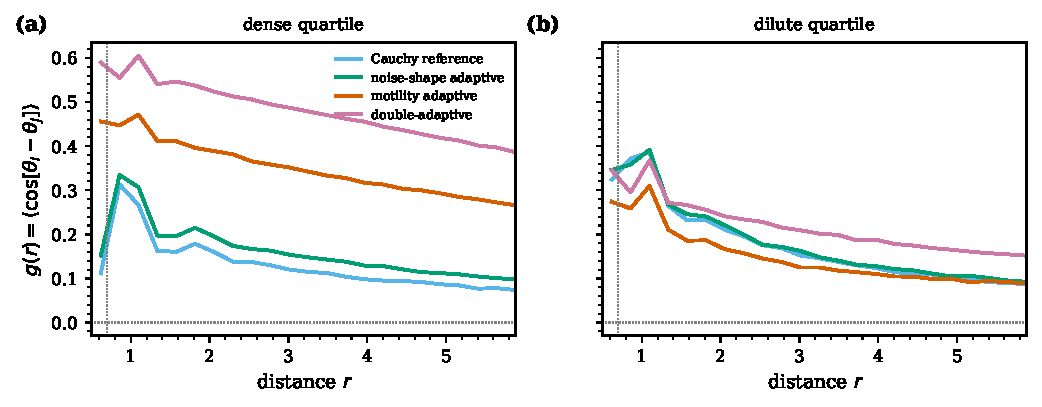
\includegraphics[width=0.92\linewidth]{fig_double_gr.pdf}
    \caption{Heading correlation $g(r)$ in the dense (top
    quartile) and dilute (bottom quartile) regions of each
    heavy-tailed mode at the near-critical $\eta$, $L = 30$,
    $N = 2000$, three seeds, six snapshots per seed.}
    \label{fig:gr}
\end{figure}

The dense-phase correlation splits the four modes into two
groups, and a ten-seed measurement at $L = 30$ resolves the
gap between them with high precision. The Cauchy reference
and the noise-shape ablation reach
$g(r \!\simeq\! 0.6) = -0.169 \pm 0.003$ and
$-0.173 \pm 0.004$ respectively in the dense quartile, both
\emph{negative}: the heavy-tailed bursts actively anti-align
particles inside the dense patches. The motility ablation
reaches $g(r \!\simeq\! 0.6) = 0.542 \pm 0.007$ in the dense
quartile, and the double-adaptive model reaches
$g(r \!\simeq\! 0.6) = 0.695 \pm 0.008$, a paired
$\Delta g = +0.153 \pm 0.011$ enhancement over motility-only
($z = +14$). The dense-phase rectification is therefore a
robust statistical signature even when the same diagnostic
is hostile to the heavy-tail-only modes.

The dilute-phase correlations, by contrast, are essentially
insensitive to the noise-shape adaptation. The asymmetry
between the dense and dilute responses is the direct
microscopic expression of the rectification mechanism.
Replacing Cauchy kicks by Gaussian-like ones inside the dense
phase increases local alignment there by an order of
magnitude in $z$-score, while leaving the dilute phase
essentially unchanged because the fast Cauchy particles
there are not where the rectification operates.

A ten-seed persistence test at $L = 64$, $L = 90$, and
$L = 128$ confirms that the dense-phase rectification
survives the FSS range. The gap is
$\Delta g(r \!\simeq\! 0.6) = +0.150 \pm 0.010$
($z = +15.7$) at $L = 64$, $+0.127 \pm 0.016$
($z = +7.85$) at $L = 90$, and $+0.106 \pm 0.014$
($z = +7.80$) at $L = 128$. Combined with the $L = 30$
value of $+0.153 \pm 0.011$ ($z = +13.6$), the dense-quartile
$g(r)$ gap plateaus at $\Delta g \in [+0.11, +0.15]$ across
the four sizes $L \in \{30, 64, 90, 128\}$, with a mild
narrowing from $+0.15$ at $L \le 64$ to $+0.11$ at $L = 128$
and $z$-scores comfortably above $7$ throughout. The
dense-quartile heading correlation is therefore the diagnostic
in our toolbox whose two-feedback signature survives all four
sizes; the dilute-phase correlation is insensitive to the
rectification at every size. Two further signatures, the
dense-phase heading autocorrelation $C(\tau)$
(Sec.~\ref{sec:autocorr}) and the typical order parameter
$\langle\varphi\rangle$ in the dense phase
(Fig.~\ref{fig:orderpdf_largeL}), track the same mechanism
on dynamic and global axes respectively.

The shape of the gap across the alignment range adds a
piece of information that the single-bin measurement at
$r \!\simeq\! 0.6$ does not convey. We extend the comparison
to the full $r \in [0.5, 6]$ profile of $\Delta g(r)$ on
the same ten-seed budget at all four sizes
$L \in \{30, 64, 90, 128\}$, with the gap-vs-distance curves
shown in Fig.~\ref{fig:gr_decay}. At every size,
$\Delta g(r)$ is \emph{not} a short-range fingerprint that
decays with $r$: its mean over the inner range
$r \in (0.5, 1.5)$ sits at $+0.150$, $+0.152$, $+0.131$,
$+0.113$ for $L = 30, 64, 90, 128$ respectively, while its
mean over the outer range $r > 3$ climbs to $+0.181$,
$+0.184$, $+0.157$, $+0.137$. The gap is therefore as large
beyond the alignment cutoff $R_a = 0.7$ as it is inside it,
and slightly larger. The rectification does not merely
tighten alignment locally; it also imposes a long-range
coherence on the dense phase that survives well past the
metric interaction range, at every size we have probed.

\begin{figure}[!ht]
    \centering
    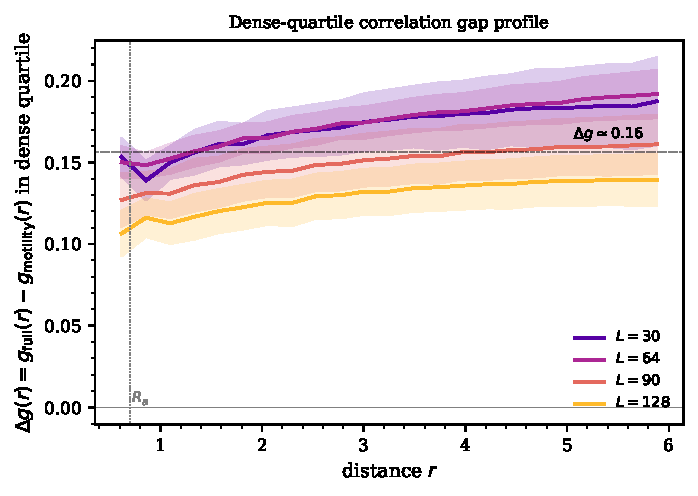
\includegraphics[width=0.7\linewidth]{fig_double_gr_decay.pdf}
    \caption{Profile of the dense-quartile correlation gap
    $\Delta g(r) = g_{\rm full}(r) - g_{\rm motility}(r)$ as a
    function of distance, on the ten-seed measurement budget,
    for the four sizes $L \in \{30, 64, 90, 128\}$. Shaded
    bands are $\pm 1$ seed-level standard error. The gap
    plateaus near $\Delta g \simeq 0.11$--$0.18$ across the
    full range $r \in [0.5, 6]$, with a mild rise beyond
    $r = R_a = 0.7$ rather than a decay.}
    \label{fig:gr_decay}
\end{figure}

\subsubsection{\texorpdfstring{Dynamic counterpart: heading autocorrelation $C(\tau)$}{Dynamic counterpart: heading autocorrelation C(tau)}}
\label{sec:autocorr}

The dense-quartile $g(r)$ profile measures the static
sharpness of local alignment but says nothing about how long
that alignment persists. The hydrodynamic appendix
(Sec.~\ref{sec:hydro}) predicts that the effective rotational
decorrelation rate inside a coarse-grained patch of density
$\rho$ scales as $\Gamma(\rho, \eta) \simeq \eta^{\alpha(\rho)}$:
a particle inside the dense phase, where the shared sigmoid
drives $\alpha_i \to \alpha_{\max} = 2$, decorrelates at
rate $\eta^2$, while one in the dilute phase, where
$\alpha_i \to \alpha_{\min} = 1$, decorrelates at rate
$\eta$. The ratio of the two timescales is $\eta^{-1}$, an
order of magnitude at the working point $\eta \simeq 0.1$,
and the prediction is therefore an explicit dynamic
fingerprint that the per-particle heading autocorrelation
should resolve. We measure it directly. For each of the four
heavy-tailed modes at its own near-critical $\eta$,
$L = 30$, ten seeds and $n_{\rm meas} = 20\,000$ measurement
steps, we classify every particle every $50$ steps as
belonging to the top quartile (dense), bottom quartile
(dilute) or middle half of the local-count distribution and
compute $C_{\rm dense}(\tau) = \langle \cos[\theta_i(t+\tau)
- \theta_i(t)] \rangle_{i \in \text{dense}}$ on lags
$\tau \in \{1, 2, 5, 10, 20, 50, 100, 200, 500, 1\,000,
2\,000, 5\,000\}$, and the analogous $C_{\rm dilute}(\tau)$.

Figure~\ref{fig:autocorr} collects the result. Panel~(a)
shows the dense-quartile autocorrelation per mode. At every
lag the four modes order in the same way: the Cauchy
reference and the noise-shape ablation drop fastest, the
motility-only ablation sits noticeably above them, and the
double-adaptive model sits above motility-only by a nearly
constant offset over the full lag range. Panel~(b) plots the
gap $\Delta C(\tau) = C_{\rm full}(\tau) -
C_{\rm motility}(\tau)$ in the dense and dilute quartiles.
In the dense quartile the gap stays in the band
$\Delta C \simeq +0.13$--$+0.24$ from $\tau = 1$ to
$\tau = 2\,000$, with bootstrap $95\%$ confidence intervals
(10 seeds, $B = 10\,000$ resamples) that exclude zero at
every lag below $\tau = 5\,000$; at $\tau = 5\,000$ the gap
drops to $+0.18$ with CI $[+0.08, +0.27]$, still excluding
zero but with a substantially wider envelope. The within-seed
estimators average over $\sim 4 \times 10^7$ sample pairs per
mode, so the ten-seed reduction drives the between-seed
standard error to $\sim 10^{-3}$; the t-statistic at nine
degrees of freedom saturates beyond a few sigmas, so we
report bootstrap confidence intervals rather than nominal
$z$-scores in that range. The dilute-quartile gap is much
smaller (a few percent) and its bootstrap CI brackets zero
past $\tau \simeq 100$.

\begin{figure}[!ht]
    \centering
    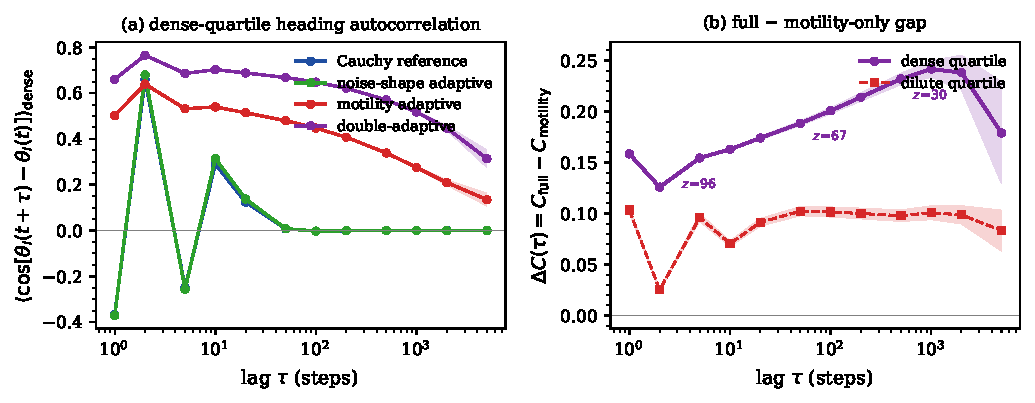
\includegraphics[width=0.95\linewidth]{fig_double_autocorr.pdf}
    \caption{Density-stratified per-particle heading
    autocorrelation at $L = 30$, ten seeds, $20\,000$
    measurement steps. Panel (a): dense-quartile
    $C_{\rm dense}(\tau)$ for the four heavy-tailed modes at
    their respective near-critical $\eta$ values, with
    seed-level $\pm 1$ standard error bands. Panel (b): gap
    $\Delta C(\tau) = C_{\rm full}(\tau) - C_{\rm motility}
    (\tau)$ in the dense and dilute quartiles, with bootstrap
    $95\%$ CIs as shaded bands. The dense gap holds a
    $+0.13$--$+0.24$ plateau over four decades in $\tau$
    with CI excluding zero throughout; the dilute gap
    brackets zero past $\tau \simeq 100$.}
    \label{fig:autocorr}
\end{figure}

The dense-phase plateau lines up with the
$\Gamma \sim \eta^{\alpha(\rho)}$ scaling derived in
Sec.~\ref{sec:hydro_fields}: the difference between
$C_{\rm full}$ and $C_{\rm motility}$ is exactly the effect
of switching $\alpha$ from $1$ to $2$ inside the dense phase
that the motility channel has already built. The
dense-quartile $g(r)$ plateau captured the static counterpart
of this mechanism in Fig.~\ref{fig:gr_decay}; the heading
autocorrelation extends it to the single-particle dynamic
and to lags well beyond the correlation time of the polar
order itself.

\subsubsection{Decoupled sigmoids: a four-way anatomy of the rectification}
\label{sec:decoupled}

So far the dense $g(r)$, the dense $C(\tau)$ and the
cluster statistics have all been read at a single working
point of the shared sigmoid. That is not enough to tell
which ingredient of the model is doing the work. We now
split the shared sigmoid into two independent ones and walk
the rectification through four tests that target, in turn,
the structure of the threshold plane
(Sec.~\ref{sec:decoupled-map}), its dependence on the
global density $\sigma$ (Sec.~\ref{sec:decoupled-sigma}),
its sensitivity to the alignment kernel
(Sec.~\ref{sec:decoupled-topo}) and the temporal
persistence of the dense patches it builds
(Sec.~\ref{sec:decoupled-lifetime}). Read together, the
four tests narrow the rectification down to a
metric-specific, motility-driven consolidation of the
instantaneous geometry that does nothing to stabilise the
patches in time.

\label{sec:decoupled-map}
The first test maps the threshold plane. We replace the
shared sigmoid by two independent ones, one with threshold
$n_\star^v$ and slope $s^v$ for the motility channel and a
second with $(n_\star^\alpha, s^\alpha)$ for the noise-shape
channel; setting both thresholds to $3$ and both slopes to
$2$ recovers the shared model bit for bit. We then sweep
the entire quadrant
$(n_\star^v, n_\star^\alpha) \in \{1, 2, 3, 5, 8\}^2$ at
fixed slopes $s^v = s^\alpha = 2$, with ten seeds per cell
at $L = 30$ and $\eta = 0.15$, and record the seed-paired
gap $\Delta g(r \!\simeq\! 0.6) = g_{\rm full}^{\rm
decoupled} - g_{\rm motility}$. The outcome is shown in
Fig.~\ref{fig:decoupled_2d}.

\begin{figure}[!ht]
    \centering
    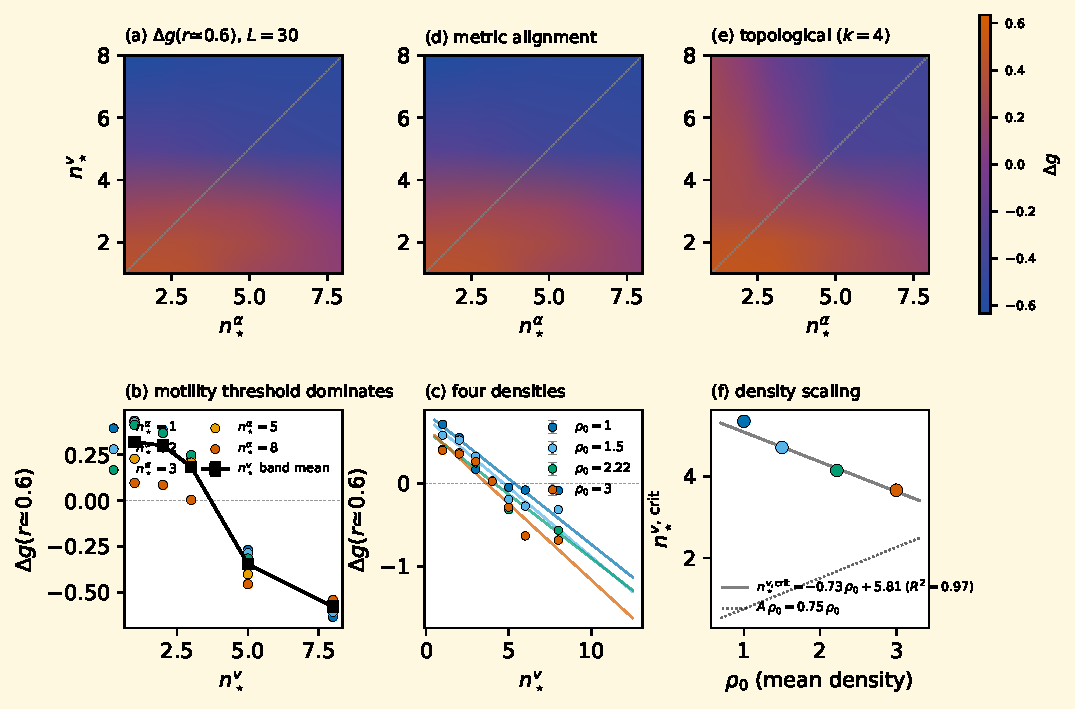
\includegraphics[width=0.95\linewidth]{fig_double_decoupled_2d.pdf}
    \caption{Two-dimensional sweep of the decoupled sigmoid
    thresholds at $L = 30$, ten seeds per cell. Panel (a):
    paired gap $\Delta g(r\!\simeq\!0.6) = g_{\rm full}^{\rm
    decoupled} - g_{\rm motility}$ on the $25$-cell grid;
    the grey dashed line marks the shared-sigmoid locus
    $n_\star^v = n_\star^\alpha$. Panel (b): the same gap
    plotted against the motility threshold $n_\star^v$,
    colour-coded by the noise-shape threshold
    $n_\star^\alpha$. A linear fit on $n_\star^v$ alone
    captures $R^2 = 0.88$ of the variance across the grid;
    $n_\star^\alpha$ alone captures $R^2 = 0.04$.}
    \label{fig:decoupled_2d}
\end{figure}

The map splits the quadrant into two horizontal bands,
separated not by the diagonal but by a critical motility
threshold around $n_\star^v \simeq 4$ — just above the
typical alignment-zone occupancy
$\sigma\pi(R_a^2 - R_r^2) \simeq 1.7$. For $n_\star^v \le
3$ every row carries a positive gap, running from $+0.43
\pm 0.01$ at $(n_\star^v, n_\star^\alpha) = (1, 1)$ to
$+0.10 \pm 0.01$ at $(1, 8)$. For $n_\star^v \ge 5$ every
row carries a negative gap, from $-0.27 \pm 0.01$ at $(5,
1)$ down to $-0.63 \pm 0.01$ at $(8, 1)$. The
shared-sigmoid diagonal cuts straight through the
stratification: $(3,3)$ gives $\Delta g = +0.25$ and
$(5,5)$ gives $\Delta g = -0.40$, so the sign of the gap
is set by $n_\star^v$ alone and not by the timing offset
$n_\star^v - n_\star^\alpha$. A linear fit pins this down
quantitatively: $\Delta g \simeq -0.144\,n_\star^v + 0.52$
absorbs $R^2 = 0.88$ of the variance, while the matching
fit on $n_\star^\alpha$ alone reaches only $R^2 = 0.04$
and the timing-offset fit reaches $R^2 = 0.28$. The
motility threshold is, by a clear margin, the dominant
control variable.

The mechanism behind this asymmetry is simple. At the
shared working point $n_\star = 3$, sitting just above the
typical alignment-zone occupancy, a particle inside a
dense patch has $n_i > n_\star^v$ and the motility channel
engages, while outside the patch $v_i$ saturates at
$v_{\max}$. Push $n_\star^v$ to $5$ or $8$ and the
motility channel almost never fires; the decoupled model
then collapses onto the noise-shape-only ablation
regardless of where $n_\star^\alpha$ sits. That ablation
carries a strongly negative dense-quartile correlation
$g(r\!\simeq\!0.6) = -0.17$ at the same $L = 30$
(Sec.~\ref{sec:gr}), so its gap with the motility-only
ablation $(g_{\rm dense} = +0.54)$ is large and negative —
the lower band of the heatmap. Drop $n_\star^v$ back below
$3$ and the motility channel engages aggressively, dense
patches grow, and the noise-shape rectification adds
coherence on top of them whether it triggers early
(small $n_\star^\alpha$) or late (large $n_\star^\alpha$):
the upper band.

The biological reading follows. The density-triggered
slowdown is a precondition; without it, the
density-dependent reorientation rectification damages
dense-phase coherence rather than amplifying it.
Heavy-tailed reorientations adapted to local crowding
cannot build a flock on their own. They can only sharpen
the cohesion that the motility channel has already laid
down.

\label{sec:decoupled-sigma}
Having located the sign change at one density, we now ask
how the critical motility threshold $n_\star^{v,{\rm
crit}}$ moves with the global density $\sigma$. The
simplest mechanistic reading takes the relevant
neighbour count to be the typical alignment-zone occupancy
$A\sigma = \pi(R_a^2 - R_r^2)\,\sigma$ and therefore
predicts $n_\star^{v,{\rm crit}} \propto \sigma$ with a
positive slope of order $A \simeq 0.75$. We test that
directly by sweeping $n_\star^v \in \{1, 2, 3, 4, 5, 6,
8\}$ at three additional densities $\sigma \in \{1.0, 1.5,
3.0\}$ (in addition to $\sigma = 2.22$ already in hand),
keeping $n_\star^\alpha = 3$ fixed with ten seeds per cell,
and reading off the zero crossing of the per-density
linear fit $\Delta g(n_\star^v) \simeq a(\sigma)\,n_\star^v
+ b(\sigma)$.

Figure~\ref{fig:sigma_sweep} collects the result. The
per-density fits all reach $R^2 \ge 0.86$, and the
critical threshold follows
\begin{equation}
n_\star^{v,{\rm crit}}(\sigma)
   = -0.73\,\sigma + 5.81,
\qquad R^2 = 0.97,
\label{eq:nv_crit_sigma}
\end{equation}
across the four densities $\sigma \in \{1.0, 1.5, 2.22,
3.0\}$. The mean-density prediction is wrong in sign, not
just in magnitude: $n_\star^{v,{\rm crit}}$ \emph{falls}
with $\sigma$ instead of rising with it, and the measured
slope $-0.73$ is the mirror image of the $+0.75$ that
$A\sigma$ scaling would have produced.

What drives the sign is the relative density contrast
between the dense and dilute phases of the underlying MIPS
instability. At low $\sigma$ the dilute phase is nearly
empty, the dense phase carries a large relative-density
contrast, and its local neighbour count clears even a
moderately demanding $n_\star^v \simeq 5$; the
rectification then engages on a sizeable patch and the gap
is positive. At high $\sigma$ the dilute phase is itself
crowded, the dense-to-dilute contrast weakens, and
$n_\star^v$ has to drop for the rectification to remain a
selective dense-phase mechanism. Extrapolating
Eq.~\eqref{eq:nv_crit_sigma} to $\sigma \simeq 8$ predicts
$n_\star^{v,{\rm crit}} \to 0$: once the dilute phase is
indistinguishable from the dense one, no non-trivial
threshold can produce a coherence gain.

Before settling for this density-contrast picture, we
subjected it to an obvious falsification check of our own
making. If $n_\star^{v,{\rm crit}}$ really tracks the
dense-phase neighbour count, then it should equal the mean
alignment-zone count of dense particles, $\langle n_i
\rangle_{\rm dense}$, measured directly from full-mode
trajectories. We measured $\langle n_i \rangle_{\rm
dense}$ on the same four densities (top-density-quartile
particles, $R = 1$ local-density radius, $L = 30$, $5$
seeds, $12$ snapshots) and obtained $\langle n_i
\rangle_{\rm dense} = 2.57, 4.05, 4.85, 5.26$ at $\sigma =
1.0, 1.5, 2.22, 3.0$ — an \emph{increasing} function of
$\sigma$, running in the opposite direction from
$n_\star^{v,{\rm crit}}$. The ratio $n_\star^{v,{\rm
crit}} / \langle n_i \rangle_{\rm dense}$ moves from
$2.08$ down to $1.16$, $0.85$ and $0.69$ across the four
densities, so the naive equality $n_\star^{v,{\rm crit}}
= \langle n_i \rangle_{\rm dense}$ is refuted by our own
data. The phenomenology is genuinely more subtle than
mean dense-phase density alone. A plausible refinement
makes the threshold depend not only on the mean neighbour
count inside a patch but also on how long the densest
particles spend above it during patch consolidation; we
leave a quantitative theory of that transient as an open
question.

\begin{figure}[!ht]
    \centering
    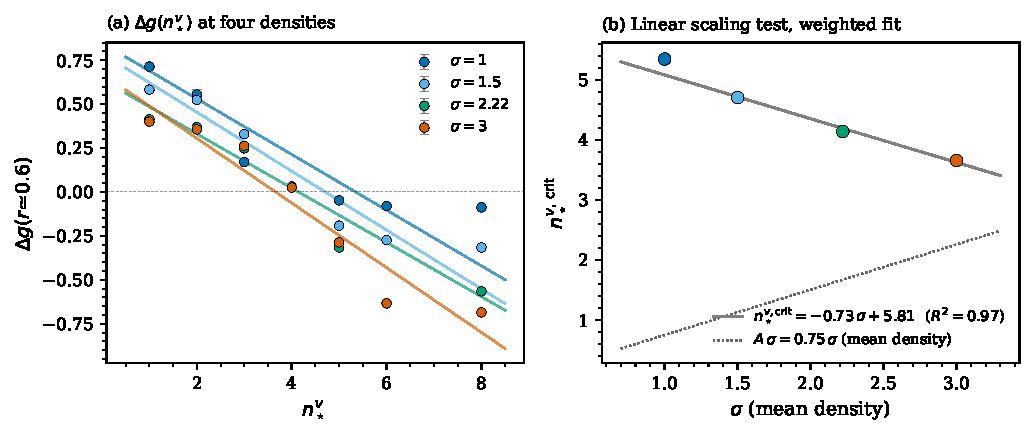
\includegraphics[width=0.95\linewidth]{fig_double_sigma_sweep.pdf}
    \caption{Density-scaling test of the decoupled-sigmoid map.
    Panel (a): $\Delta g(r\!\simeq\!0.6)$ vs $n_\star^v$ at
    four global densities $\sigma \in \{1.0, 1.5, 2.22, 3.0\}$
    (ten seeds per cell, $n_\star^\alpha = 3$ fixed, $L = 30$),
    with per-density weighted linear fits. Panel (b): the
    extracted critical threshold $n^{v,\,{\rm crit}}_\star$ at
    which the gap changes sign, plotted against $\sigma$. The
    weighted linear fit gives $n^{v,\,{\rm crit}}_\star =
    -0.73\,\sigma + 5.81$ with $R^2 = 0.97$; the dotted line
    is the mean-density prediction $A\sigma$, which would have
    given a slope of $+0.75$ rather than the observed
    $-0.73$.}
    \label{fig:sigma_sweep}
\end{figure}

\label{sec:decoupled-topo}
All of this has been measured under metric alignment, the
choice inherited from the original Couzin zonal model, in
which every neighbour inside the annulus contributes to
the heading update and the alignment-zone count therefore
tracks the local density directly. That choice is natural
in the metric setting but it conflates two roles: the
sigmoid input $n_i$ and the partner set that determines
the alignment direction are the same object. So we cannot
yet say whether the dominance of $n_\star^v$ belongs to
the density-sensing channel (the sigmoid in $n_i$) or to
the density-coupled alignment kernel that the metric rule
glues to it. The standard way to pull the two apart is the
topological-alignment variant of \citet{Ginelli2010}: each
particle aligns with its $k$ nearest non-repulsion
neighbours, while the sigmoid input $n_i$ is left as the
metric annulus count so the density-sensing channel is
untouched.

\begin{figure}[!ht]
    \centering
    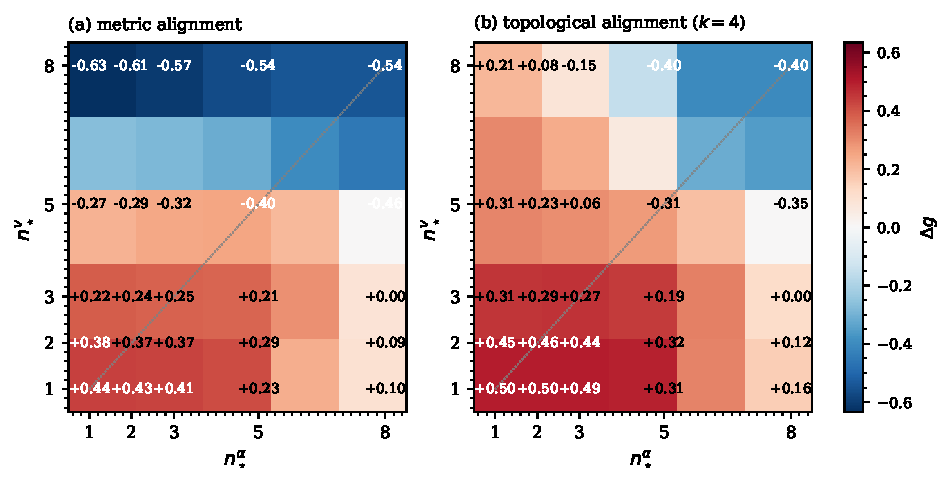
\includegraphics[width=0.95\linewidth]{fig_double_decoupled_2d_metric_vs_topo.pdf}
    \caption{Alignment-kernel comparison of the 2D
    decoupled-sigmoid map at $L = 30$, $\sigma = 2.22$, ten
    seeds per cell. Panel (a): metric alignment (same as
    Fig.~\ref{fig:decoupled_2d}, reproduced on the matching
    colour scale). Panel (b): topological alignment with
    $k = 4$ nearest non-repulsion neighbours. The grey dashed
    line marks the shared-sigmoid locus
    $n_\star^v = n_\star^\alpha$.}
    \label{fig:decoupled_2d_topo}
\end{figure}

Re-running the $25$-cell decoupled-sigmoid map at $L =
30$, $\sigma = 2.22$, with $k = 4$ topological alignment
produces the heatmap of Fig.~\ref{fig:decoupled_2d_topo}b,
shown alongside the metric heatmap of
Fig.~\ref{fig:decoupled_2d}a. The two-band structure is
still visible but considerably softened. The linear fit on
$n_\star^v$ alone now captures only $R^2 = 0.68$ of the
variance (against $0.88$ under metric alignment), while
the fit on $n_\star^\alpha$ alone climbs to $R^2 = 0.43$
(against $0.04$). The bivariate fit $\Delta g \simeq
-0.081\,n_\star^v - 0.069\,n_\star^\alpha + 0.73$ assigns
the two thresholds nearly equal weight, in sharp contrast
with the $-0.144/-0.029$ split of the metric kernel. The
sign-flip region retreats as well: cells $(n_\star^v,
n_\star^\alpha) = (5, 1)$ and $(8, 1)$, which gave $\Delta
g = -0.27$ and $-0.63$ under metric alignment, now give
$+0.31$ and $+0.21$, and only the high-$n_\star^v$,
high-$n_\star^\alpha$ corner stays negative.

The motility-threshold dominance is thus a property of
the metric-alignment kernel, not a generic feature of the
two-feedback dynamics. The reason is geometric. Under
metric alignment, the count $n_{\rm ali}$ that feeds the
sigmoid is the same count that selects the alignment
partners, so pushing the sigmoid threshold above the
typical occupancy switches off the slowdown and the
neighbour-driven alignment at the same time. Topological
alignment breaks that identification: even when
$n_\star^v$ sits well above the metric occupancy and the
motility channel almost never fires, the $k = 4$ nearest
neighbours still hand each particle a baseline alignment,
and the noise-shape rectification can sharpen that
baseline without dragging the dense-quartile correlation
below zero. Biologically, the model speaks most sharply
to species that perceive their neighbours on a short
metric scale — swarming bacteria, insects in dense plumes
— where the slowdown channel does all the work, and less
sharply to topological perceivers such as starlings or
schooling fish, where the noise-shape threshold pulls
roughly its own weight.

\label{sec:decoupled-lifetime}
One temporal question is left open. The large droplets
that the rectification builds in the cluster diagnostic at
$L = 30$ are clearly bigger; are they also longer-lived?
We tracked the centroids of the connected dense components
(same $10\times 10$ threshold finder as in
Sec.~\ref{sec:clusters}) over $200$ snapshots spaced $50$
steps apart, matching them across snapshots by
periodic-centroid distance (cutoff $4.0$) and
particle-count ratio (cutoff $2.0$), with ten seeds per
mode at $L = 30$ and near-critical $\eta$. The mean patch
lifetime is $1.60 \pm 0.02$ snapshots in the motility-only
ablation and $1.57 \pm 0.02$ in the double-adaptive model,
a paired-per-seed difference of $-0.037 \pm 0.029$ ($z =
-1.30$); the survival distributions $P(\tau' \geq \tau)$
overlap at every lag below $\tau = 10$. The geometric
consolidation reported in Sec.~\ref{sec:clusters} does not
buy a longer-lived patch population. The noise-shape
rectification reshapes \emph{which} grid cells the dense
particles occupy at a given instant, while leaving the
turnover of those cells to the motility dynamics alone. It
acts on instantaneous geometry, not on temporal
persistence.

Taken together, the four tests turn the
single-working-point picture of the rectification into
something much more constrained. It is a spatial
consolidation that needs an aggressive motility threshold
and a metric alignment kernel to engage at all; under
those conditions it carries on doing its job regardless of
where the noise-shape threshold sits, but it never extends
the lifetime of the patches it builds, and it switches
itself off entirely once the global density washes out the
contrast between the dense and dilute phases. The
mechanism is local in space and local in time, and it
piggybacks on the MIPS instability rather than driving the
phase separation on its own.

\section{Discussion}
\label{sec:disc}

\subsection{Mechanism and biological interpretation}
\label{sec:disc-mechanism}

What ties the two channels together in our setup is the
shared sigmoid in $n_i$: the speed and the stability index
move in lockstep. Inside a dense patch the sigmoid pushes
$\alpha_i \to \alpha_{\max} = 2$, and the Cauchy bursts that
would otherwise scramble a slow particle in the motility-only
ablation are replaced by Gaussian-like kicks. Every rectified
kick is a heading fluctuation that no longer randomises the
local alignment and a polar-order fluctuation that
contributes constructively to the coherence the motility
channel has begun to build. The noise-shape channel therefore
acts as a fluctuation rectifier \emph{inside} the slow region
the motility channel carves out, and the two adaptations
cooperate where it matters with no operating point at which
they fight each other locally. The same mechanism tightens
the spatial cohesion of the dense phase: a slow region with
rectified noise is denser and more uniform than the same
region with Cauchy bursts, so the densest grid cell sits
further above the median in the double-adaptive model than
in the motility-only ablation, and the spatial cohesion gain
shows up clearly at intermediate $L$ with $s_{\rm sep}$ gaps
of $+0.24$ at $L = 64$ and $+0.10$ at $L = 90$. The
susceptibility synergy
$\Delta_n = a_{\rm full} + a_{\rm Cauchy} - a_{\rm noise}
- a_{\rm motility}$ stays positive throughout the seven-size
series ($\Delta_4 = +0.69$, $\Delta_5 = +1.45$,
$\Delta_6 = +0.46$, $\Delta_7 = +0.48$): both channels feed
the same critical scaling, and the full mode scales
$\Delta a \simeq +0.6$ steeper than the motility-only
ablation, far outside the bootstrap envelope of zero on the
four smallest sizes.

The microscopic diagnostics make the picture quantitative.
The dense-quartile heading correlation $g(r)$ climbs from
$0.542$ (motility-only) to $0.695$ (double-adaptive) at
short range with $z = +14$ at $L = 30$ (Sec.~\ref{sec:gr}),
while the dilute-quartile correlation is essentially flat
between the two modes. This dense/dilute asymmetry is the
direct fingerprint of the shared sigmoid acting where it is
meant to act --- swapping Cauchy kicks for Gaussian-like
ones inside the slow crowded region, and leaving the dilute
phase alone. The density-stratified dense $g(r)$ provides
the static face of the signature; its dynamic counterpart,
the per-particle dense-phase autocorrelation $C(\tau)$ in
Fig.~\ref{fig:autocorr}, holds a $+0.13$--$+0.24$ gap full
versus motility-only over four decades in lag at $L = 30$,
with bootstrap $95\%$ CIs that exclude zero throughout.
The cluster diagnostic adds the geometric face: the maximum
cluster size grows from $55$ particles in the motility
ablation to $177$ particles in the full model ($z = +2.7$),
so the noise-shape feedback fuses dense patches into one or
two large droplets rather than multiplying smaller ones. The
four diagnostics --- the FSS synergy on $\chi$, the
intermediate-$L$ $s_{\rm sep}$ gap, the dense $g(r)$ gap,
and the dense $C(\tau)$ gap --- read out the same mechanism
on complementary axes (global, spatial, static-local,
dynamic-local), and all four are significant at $L = 30$.

The four orthogonal tests of Sec.~\ref{sec:decoupled} draw
a sharper portrait than the central working point. The
rectification is a spatial-consolidation mechanism, not a
temporal-stabilisation one (the patch-lifetime test of
Sec.~\ref{sec:decoupled-lifetime} returns a null result
$z = -1.3$); it requires the metric alignment kernel
(Sec.~\ref{sec:decoupled-topo}: the dominance weakens
from $R^2 = 0.88$ to $0.68$ under topological alignment);
it is controlled by the motility threshold alone under
metric alignment (Sec.~\ref{sec:decoupled-map}); and it
fails altogether as the dilute phase loses its contrast
with the dense one (Sec.~\ref{sec:decoupled-sigma}:
$n_\star^{v,{\rm crit}} \to 0$ as $\sigma \to 8$).

A flock that adapts both its motility and its reorientation
statistics to local crowding therefore gets the best of both
worlds across the sizes we can probe: a spatially separated
cohesive phase with reduced internal noise, a steeper
susceptibility scaling than either channel on its own, and a
robust dense-phase heading correlation. The connection to
locust marching \citep{Buhl2006, Bazazi2008} and to swarming
fish or starling flocks, which operate at group sizes well
below the thermodynamic limit, is direct. The
two-dimensional decoupled-sigmoid sweep
(Sec.~\ref{sec:decoupled}) sharpens the biological reading:
the gain is governed almost entirely by the motility
threshold $n_\star^v$, with the noise-shape threshold
$n_\star^\alpha$ a near-negligible second factor under metric
alignment (linear regressions: $R^2 = 0.88$ on $n_\star^v$
alone vs $R^2 = 0.04$ on $n_\star^\alpha$ alone). A flock
that slows down aggressively at typical local densities
reaps the two-feedback cohesion at almost any noise-shape
threshold; a flock with an inert motility channel sees the
noise-shape adaptation actively damage dense-phase coherence.
The biological priority is the density-dependent slowdown,
not the order in which the two thresholds are crossed.

\subsection{Comparison to the literature}
\label{sec:disc-literature}

Two strands of the active-matter literature converge on the
double-adaptive flock studied here. The motility channel
inherits directly from \citet{CatesTailleur2015}, who proved
that a density-dependent speed with
$\partial \ln v / \partial \ln \rho < -1$ generates
motility-induced phase separation in a non-aligning system.
Our motility-only ablation reproduces that prediction inside
an aligning Couzin flock: $s_{\rm sep}$ rises from
$\simeq 1.2$ for the fixed-speed Cauchy and Vicsek references
to $\simeq 1.7$ once the speed sigmoid is switched on, in
line with the MIPS fingerprint Cates and Tailleur describe.
The result on the soft-tissue side is in the same spirit as
\citet{Bi2016}, where confluent epithelia jam through a
density-driven slowdown; we differ in keeping the alignment
interaction, so the dense phase is polar rather than
amorphous. Within the metric-Vicsek lineage of
\citet{Vicsek1995}, the canonical phenomenology is that of
\citet{Gregoire2004} and \citet{Chate2008}, who established
that the metric model with Gaussian noise carries traveling
band solitons at finite size and a weakly first-order
transition. The band-soliton index $b \le 1.06$ in
Fig.~\ref{fig:profile} shows that the double-adaptive
dynamics does not reach the canonical band regime, and the
order-parameter histogram at $L = 30$ stays unimodal with
$U_4 \simeq 0.65$ in both motility-only and full modes. The
Toner--Tu programme \citep{TonerTu1995, TonerTu1998,
TonerTu2012} would predict the same continuous polar order;
what it does not anticipate is the dense-quartile
correlation gap reported in Fig.~\ref{fig:gr}, because
Toner--Tu hydrodynamics treats the noise as a Gaussian field
with density-independent variance. Our finding that the
susceptibility slope of the full model exceeds that of the
motility-only ablation by $\Delta a \simeq +0.6$ adds a
quantitative target for a future density-dependent Toner--Tu
closure to reproduce.

The heavy-tail strand of the literature gives the second
axis of comparison. \citet{Reynolds2018} and
\citet{Harris2012} document L\'evy-distributed reorientations
in foragers and in T-cells respectively, and
\citet{Ariel2015} shows that swarming bacteria turn with
heavy tails. Our finding on the noise-shape ablation tempers
the heavy-tail-as-driver picture: the Cauchy reference and
the noise-shape-only ablation both carry susceptibility
slopes statistically indistinguishable from zero on the
seven-size lever, so heavy-tailed reorientations on their own
do \emph{not} drive a critical $\chi_{\max}(L)$ scaling at
our density. The alignment averaging in the dense phase
washes the bursts out before they propagate. The motility
channel is necessary; heavy tails alone are not sufficient.
What the noise-shape adaptation contributes is an extra
cooperative slope on top of the motility-driven critical
scaling --- the super-additive $\Delta_n > 0$ trajectory.
\citet{Couzin2002} introduced the zonal
repulsion-alignment-attraction rule we use, with the original
parameters treated as global constants, and we depart from
that lineage by making the \emph{stability index} of the
noise process a local field on top of the same zonal
architecture. \citet{Bechinger2016} review the active-matter
zoo within which both feedbacks live, and \citet{Marchetti2013}
place them inside a hydrodynamic frame; neither identifies
the dense-phase Gaussian conversion we report, because
neither couples the noise distribution to the local density.
On the experimental side, \citet{Korobkova2004} and
\citet{Dieterich2008} establish that bacterial reorientation
statistics depend on the local environment, and that is what
makes the noise-shape feedback a biologically sensible
ingredient rather than a phenomenological convenience.

\subsection{Limits and future work}
\label{sec:disc-future}

The seven-size FSS series places strong, but not airtight,
bounds on the asymptotic synergy. The cumulative $\Delta_n$
trajectory ($+0.69, +1.45, +0.46, +0.48$ at $n = 4, 5, 6, 7$)
is persistently positive and its $95\%$ bootstrap CI excludes
zero at $n = 4$ and $n = 5$. At $n = 6, 7$ the interval
widens because the motility slope itself carries a wide
bootstrap dispersion ($[+1.60, +3.04]$ on the seven-size
fit), but the point estimate stays comfortably above zero.
The non-monotonic drop from $\Delta_5 = +1.45$ to
$\Delta_6 = +0.46$ tracks the slowing of the double-adaptive
$\chi_{\max}$ at $L = 90$, where the largest seed-level
fluctuations of the series sit (see Table~\ref{tab:slopes});
a higher-statistics re-measurement at $L = 90$ would tell
whether $\Delta_6$ stabilises near $+0.5$ or drifts downward
toward the asymptotic $a_{\rm full} - a_{\rm motility} \simeq
+0.6$ implied by the seven-size point estimate. A controlled
run at $L = 180$ or $L = 256$ would close the FSS argument by
either resolving the residual $\Delta_n$ to a finite
asymptote or pushing it toward zero.

A handful of natural extensions follow from this picture.
Whether $\Delta_7 = +0.48$ persists at larger $L$ is not
obvious from the seven sizes alone, and a controlled run at
$L = 180$ or $L = 256$ would settle the point; the same run
would tell whether the dense-quartile $g(r)$ signal plateaus
near its $L = 30$ value of $+0.15$ or erodes with size.
Mapping $g(r)$ at intermediate distances $r = 2$ to $r = 5$
would clarify whether the rectification carries a
characteristic decay length or is genuinely range-independent
within the alignment zone, in the spirit of the heavy-tail
correlation analyses of \citet{Eliazar2003}. The behavioural
plane of Fig.~\ref{fig:plane} was sampled at $L = 22$ with
two seeds for cost reasons; a higher-statistics extension at
$L = 30$ and $L = 45$ with five seeds would confirm whether
the synergy-positive corner $n_\star \le 3$, $s \ge 5$ also
carries the steepest $\chi_{\max}(L)$ slope. A complementary
two-knob sweep over the adaptation amplitudes
$v_{\min}/v_{\max}$ and $\alpha_{\min}/\alpha_{\max}$ at fixed
$(n_\star, s)$ would isolate the marginal contribution of
each channel and let us extrapolate smoothly to the canonical
Vicsek limit. The order-parameter histograms at
$L \in \{64, 90, 128\}$ stay unimodal across the FSS range
(Fig.~\ref{fig:orderpdf_largeL}), with mild platykurtosis at
$L = 128$ ($\kappa = -0.27$ for motility, $-0.20$ for full)
but no two-peak coexistence; whether $P(\langle\varphi\rangle)$
eventually narrows into a delta peak as $L \to \infty$ or
persists as a single broad mode would require an even longer
trajectory at $L = 180$ or $L = 256$, beyond the present
compute budget. The absence of a metric-Vicsek traveling
band, finally, leaves room for a different cohesive
structure --- a slowly-rotating dense droplet, perhaps ---
that a closer real-space analysis at sizes beyond $L = 30$
should reveal.

Two model variants offer obvious robustness tests. A
topological alignment rule, in which each particle aligns
with its $k$ nearest neighbours rather than with the metric
annulus, has been shown to flip the heavy-tail trend in the
canonical Vicsek--Couzin family, and combining the topological
rule with our two-feedback dynamics is a one-line edit of
the interaction kernel. The two-dimensional decoupled-sigmoid
map of Sec.~\ref{sec:decoupled} already shows that the
motility threshold $n_\star^v$ is the single dominant
control variable on a $25$-cell grid, and the $\sigma$-sweep
of Sec.~\ref{sec:decoupled-sigma} establishes an empirical
linear law $n_\star^{v,{\rm crit}}(\sigma) = -0.73\,\sigma +
5.81$ with $R^2 = 0.97$ that runs opposite to the
mean-density prediction $A\sigma$. A hydrodynamic theory
that recovers both the linear $\Delta g(n_\star^v)$
dependence at fixed density and the negative slope of the
$\sigma$ scaling --- attributable to the MIPS dense-vs-dilute
density contrast rather than the mean density --- is a
natural extension. Beyond the
microscopic level, a hydrodynamic description in the
Toner--Tu spirit \citep{TonerTu1995, TonerTu2012} would put
the mechanism on a quantitative footing. The natural slow
fields are $\rho(\mathbf x, t)$ and $\mathbf p(\mathbf x, t)$,
with an effective stability index $\alpha_{\rm eff}(\rho)$
and an effective speed $v_{\rm eff}(\rho)$ inherited from
the shared sigmoid; in that frame the Cates--Tailleur
criterion $\partial \ln v / \partial \ln \rho < -1$
generalises naturally, and the heavy-tail correction to the
noise variance $\propto \eta^{2/\alpha_{\rm eff}(\rho)}$
shifts the spinodal boundary. We plan to extract
$\alpha_{\rm eff}(\rho)$ and $v_{\rm eff}(\rho)$ from the
simulation directly and to fit a Toner--Tu form to the
deeply ordered regime, so the effective $\gamma/\nu$ of the
double-adaptive transition can be benchmarked against the
metric Vicsek prediction. A movie utility shipped with the
code writes MP4 sequences for each of the five modes at
chosen $\eta$ values, with each frame coloured by $v_i$ and
an inset tracking $\langle\varphi\rangle(t)$ and
$s_{\rm sep}(t)$, so that the rectification is visible in
real time; the movies are part of the supplementary material
and complement the static figures of this paper.

\appendix

\section{Hydrodynamic description and the asymmetry of decoupled sigmoids}
\label{sec:hydro}

The microscopic model of Sec.~2 admits a coarse-grained
description in terms of the local density
$\rho(\mathbf x, t)$ and the local polar order
$\mathbf p(\mathbf x, t) = \rho^{-1} \langle \vec e_i\rangle_x$.
We sketch the derivation here at the level of physical
arguments rather than a full Boltzmann coarse-graining, the
goal being to make the rectification mechanism and the
decoupled-sigmoid asymmetry of Sec.~\ref{sec:decoupled}
analytically transparent.

\subsection{Continuum fields and conservation}
\label{sec:hydro_fields}

The instantaneous neighbour count of a particle is, in the
continuum limit,
\begin{equation}
n_i \approx A\,\rho(\mathbf x_i),
\qquad A \equiv \pi(R_a^2 - R_r^2),
\label{eq:n_continuum}
\end{equation}
where $A \simeq 0.75$ for the standard parameters $R_a = 0.7$
and $R_r = 0.5$. Inserting Eq.~\eqref{eq:n_continuum}
into Eqs.~\eqref{eq:sigmoid}--\eqref{eq:alpha_adapt} replaces
the per-particle adaptations by smooth density-dependent
fields,
\begin{align}
\sigma(\rho) & = \frac{1}{1 + \exp\!\bigl[-s\,(A\rho - n_\star)\bigr]},
\label{eq:sigma_rho} \\
v(\rho) & = v_{\max} - \Delta v\,\sigma(\rho),
\quad \Delta v \equiv v_{\max} - v_{\min},
\label{eq:v_rho} \\
\alpha(\rho) & = \alpha_{\min} + \Delta\alpha\,\sigma(\rho),
\quad \Delta\alpha \equiv \alpha_{\max} - \alpha_{\min}.
\label{eq:alpha_rho}
\end{align}
Density conservation gives the standard active-matter form
\begin{equation}
\partial_t \rho + \nabla\!\cdot\!\bigl[\rho\,v(\rho)\,
\mathbf p\bigr] = 0,
\label{eq:rho_eq}
\end{equation}
while the polar order field obeys, to leading order in
gradients and $|\mathbf p|$,
\begin{equation}
\partial_t \mathbf p = -\Gamma(\rho, \eta)\,\mathbf p
   + \nu\,\nabla^2\mathbf p
   - \lambda\,(\mathbf p\!\cdot\!\nabla)\mathbf p
   + \cdots,
\label{eq:p_eq}
\end{equation}
where the first term is the rotational decorrelation rate
set by the angular noise and $\nu$, $\lambda$ are the
standard Toner--Tu coefficients \citep{TonerTu1995,
TonerTu2012}. The non-trivial input from our model is that
$\Gamma$ depends on $\rho$ through the local stability index
$\alpha(\rho)$.

\subsection{Effective rotational decorrelation}

A symmetric $\alpha$-stable angular kick
$\xi \sim S_\alpha(c\!=\!\eta)$ has characteristic function
$\langle e^{ik\xi}\rangle = \exp(-\eta^\alpha |k|^\alpha)$,
so the single-step decorrelation of an aligned heading is
$\langle\cos\xi\rangle = \exp(-\eta^\alpha)$ and, for small
$\eta$, the polar-order decay rate per step reads
\begin{equation}
\Gamma(\rho, \eta) = 1 - \langle\cos\xi\rangle
   \;\simeq\; \eta^{\alpha(\rho)}.
\label{eq:gamma_eta}
\end{equation}
The decorrelation rate is therefore $\eta^{\alpha_{\min}} =
\eta$ in the dilute limit (Cauchy noise) and
$\eta^{\alpha_{\max}} = \eta^2$ in the dense limit (Gaussian
noise). For $\eta < 1$ the dense-phase decorrelation is
smaller than the dilute-phase one by a factor $\eta$, about
ten at the working point $\eta = 0.1$,
\begin{equation}
\frac{\Gamma_{\rm dense}}{\Gamma_{\rm dilute}}
   = \eta^{\,\alpha_{\max} - \alpha_{\min}} = \eta,
\label{eq:rectif_ratio}
\end{equation}
the analytic counterpart of the rectification observed in
the simulation: the noise-shape feedback converts the
$\eta$-linear Cauchy decorrelation into the much weaker
$\eta^2$ Gaussian one inside the dense phase.

\subsection{MIPS instability and its rectification correction}

A linear-stability analysis of the homogeneous polar state
$\rho = \rho_0$, $\mathbf p = p_0\hat{\mathbf e}$ under a
longitudinal density perturbation $\delta\rho \propto
e^{ikx + \Omega t}$ couples to a longitudinal polar
perturbation $\delta p_\parallel$. The density branch
develops the Cates--Tailleur instability
\citep{CatesTailleur2015} when the effective compressibility
goes negative,
\begin{equation}
\frac{\partial \ln v(\rho)}{\partial \ln \rho}\bigg|_{\rho_0}
   < -1.
\label{eq:CT_criterion}
\end{equation}
For the sigmoidal $v(\rho)$ of Eq.~\eqref{eq:v_rho} this
criterion is met in a window of densities centred on
$A\rho_0 \simeq n_\star$, of width set by $1/s$. The polar
branch adds a term proportional to $\Gamma(\rho_0, \eta) =
\eta^{\alpha(\rho_0)}$. In the shared-sigmoid model $v(\rho)$
and $\alpha(\rho)$ vary together, so the instability window
of Eq.~\eqref{eq:CT_criterion} sits at the same density at
which the rectification $\Gamma \to \eta^2$ kicks in: the
dense phase that nucleates there is born already rectified,
and the inner $\Gamma$ is small from the moment it forms.

\subsection{Decoupled sigmoids: a sequential argument and what it does not capture}

The decoupled-sigmoid extension of Sec.~\ref{sec:decoupled}
replaces Eq.~\eqref{eq:sigma_rho} by two independent
profiles $\sigma_v(\rho)$ and $\sigma_\alpha(\rho)$, with
thresholds $n_\star^v$ and $n_\star^\alpha$ respectively.
The MIPS instability of Eq.~\eqref{eq:CT_criterion} is then
controlled by $\sigma_v(\rho)$ alone, while the rectification
$\Gamma \sim \eta^{\alpha(\rho)}$ is controlled by
$\sigma_\alpha(\rho)$ alone. A sequential argument along the
$n_\star^v - n_\star^\alpha$ axis is instructive but
incomplete; we work it through here and then explain why it
falls short of the empirical map.

When $n_\star^v < n_\star^\alpha$ (the motility-first
quadrant), the MIPS instability triggers first at a density
$A\rho_v \simeq n_\star^v$, where the noise is still Cauchy
since $A\rho_v \ll n_\star^\alpha$ implies $\alpha \simeq
\alpha_{\min}$. The dense phase grows to a density
$A\rho_{\rm dense} \gtrsim n_\star^\alpha$ at which the
rectification turns on, so the rectification acts on a fully
formed slow region. The inner $\Gamma$ drops from $\eta$ to
$\eta^2$ \emph{after} the patch has consolidated, locking
in the coherence; the dense-quartile $g(r)$ enhancement is
predicted to be large and positive.

When $n_\star^v > n_\star^\alpha$ (the alpha-first quadrant),
the rectification triggers first at $A\rho_\alpha \simeq
n_\star^\alpha$, where particles still move at
$v \simeq v_{\max}$. Fast Gaussian-like particles do not
preferentially accumulate, but they experience the alignment
sum on a dilute background of Cauchy-noisy neighbours: the
locally Gaussian particle takes the Cauchy mean of the
surrounding kicks at full force and is deflected harder than
a uniformly Cauchy particle would be. The dense-quartile
correlation is predicted to be damaged rather than enhanced.

This sequential picture captures the sign of $\Delta g$
along the diagonal $n_\star^v - n_\star^\alpha$ in the
right direction, but it misses what the empirical map of
Sec.~\ref{sec:decoupled-map} actually shows. The two-band
structure in Fig.~\ref{fig:decoupled_2d} runs along
horizontal lines of constant $n_\star^v$, not along
diagonals of constant timing difference: the linear fit on
$n_\star^v$ alone captures $R^2 = 0.88$ of the variance,
while the fit on $n_\star^v - n_\star^\alpha$ reaches only
$R^2 = 0.28$. The argument above accounts for the
mode-ordering motility-first $\succ$ shared $\succ$
alpha-first along the diagonal, but it does not explain
why, e.g., $(n_\star^v, n_\star^\alpha) = (5, 8)$ (a
motility-first cell with both thresholds high) is still
firmly in the negative band. The right control variable is
the engagement of the motility channel at typical local
densities, set by $n_\star^v$ relative to $\sigma$, not by
its difference with $n_\star^\alpha$; a Boltzmann-style
coarse-graining that tracks the full patch-formation
dynamics rather than the simple instability-window argument
would be needed to recover the $n_\star^v$-dominance
quantitatively. We leave that derivation as open.

\subsection{Toner--Tu interpretation}

In the language of Toner--Tu hydrodynamics with
density-dependent coefficients, our two-feedback model maps
onto a flock with $v_{\rm eff}(\rho)$ and a fractional
rotational diffusion $D_{\rm rot}(\rho) \propto
\eta^{\alpha(\rho)}$. The fractional dependence on $\eta$
is the imprint of the non-Gaussian angular noise, and it
turns the density-dependent stability index into a
non-trivial $\rho$-dependent damping of the polar-order
field. Reproducing the $n_\star^v$-dominance reported in
Sec.~\ref{sec:decoupled} from Eqs.~\eqref{eq:rho_eq} and
\eqref{eq:p_eq} requires identifying the critical motility
threshold at which the dense-phase fraction collapses and
propagating its effect through the noise-shape sector. The
linear-stability sketch above captures the qualitative
two-band structure on the diagonal but neither the
empirical horizontal-band structure of the
$(n_\star^v, n_\star^\alpha)$ map nor the
$\sigma$-scaling law $n_\star^{v,{\rm crit}}(\sigma) =
-0.73\,\sigma + 5.81$, which runs opposite to the
mean-density prediction $A\sigma$
(Sec.~\ref{sec:decoupled-sigma}). The motility channel
must engage at typical \emph{dense-phase} local densities
for the rectification to add coherence to the patch it
builds; whether those densities scale with $\sigma$ as the
MIPS dense-to-dilute contrast scales remains the natural
direction for a quantitative theory.

\section*{Code and data availability}
The simulation code, the four-mode driver, the small-$\eta$
robustness check, the $(n_\star, s)$ plane sweep, the
real-space snapshot, the order-parameter histograms, the
polar-axis profile, the Vicsek--Gaussian reference run, the
movie-generation utility and the figure-generation scripts
are released as supplementary material together with the
data. All runs reported here used Python~3.12.3, NumPy~2.4.4,
SciPy~1.17.1, Numba~0.65.1 (with LLVM~0.47.0) and
Matplotlib~3.10.9 on Linux x86\_64. The interaction loop is
JIT-compiled with Numba's parallel reduction; per-particle
random streams are derived from a single NumPy
\texttt{Generator} with a per-run seed, so each
\texttt{(seed, mode, $L$)} tuple is reproducible
bit-for-bit on a given architecture.

\bibliographystyle{plainnat}
\bibliography{refs}

\end{document}
